% -*- Mode:TeX -*-

%% IMPORTANT: The official thesis specifications are available at:
%%            http://libraries.mit.edu/archives/thesis-specs/
%%
%%            Please verify your thesis' formatting and copyright
%%            assignment before submission.  If you notice any
%%            discrepancies between these templates and the 
%%            MIT Libraries' specs, please let us know
%%            by e-mailing thesis@mit.edu

%% The documentclass options along with the pagestyle can be used to generate
%% a technical report, a draft copy, or a regular thesis.  You may need to
%% re-specify the pagestyle after you \include  cover.tex.  For more
%% information, see the first few lines of mitthesis.cls. 

%\documentclass[12pt,vi,twoside]{mitthesis}
%%
%%  If you want your thesis copyright to you instead of MIT, use the
%%  ``vi'' option, as above.
%%
%\documentclass[12pt,twoside,leftblank]{mitthesis}
%%
%% If you want blank pages before new chapters to be labelled ``This
%% Page Intentionally Left Blank'', use the ``leftblank'' option, as
%% above. 

\documentclass[12pt,twoside]{mitthesis}
\usepackage{lgrind}

\usepackage{graphicx}
\graphicspath{{images/}}

%tables
\usepackage{multirow}
\usepackage{booktabs}
\usepackage{array}

\newcommand{\mcrot}[4]{\multicolumn{#1}{#2}{\rlap{\rotatebox{#3}{#4}~}}} 


\newcommand*{\twoelementtable}[3][l]%
{%  
    \renewcommand{\arraystretch}{0.8}%
    \begin{tabular}[t]{@{}#1@{}}%
        #2\tabularnewline
        #3%
    \end{tabular}%
}

\usepackage{setspace}

\usepackage[colorlinks]{hyperref}
\hypersetup{colorlinks,
  citecolor=blue,
  linkcolor=blue,
  urlcolor=blue}
  
\usepackage{tabto}
  
%% These have been added at the request of the MIT Libraries, because
%% some PDF conversions mess up the ligatures.  -LB, 1/22/2014
\usepackage{cmap}
\usepackage[T1]{fontenc}
\pagestyle{plain}

%% This bit allows you to either specify only the files which you wish to
%% process, or `all' to process all files which you \include.
%% Krishna Sethuraman (1990).

%\typein [\files]{Enter file names to process, (chap1,chap2 ...), or `all' to
%process all files:}
%\def\all{all}
%\ifx\files\all \typeout{Including all files.} \else \typeout{Including only \files.} \includeonly{\files} \fi

\setlength\parindent{0pt}

\begin{document}
\let\cleardoublepage\clearpage
% -*-latex-*-
% 
% For questions, comments, concerns or complaints:
% thesis@mit.edu
% 
%
% $Log: cover.tex,v $
% Revision 1.8  2008/05/13 15:02:15  jdreed
% Degree month is June, not May.  Added note about prevdegrees.
% Arthur Smith's title updated
%
% Revision 1.7  2001/02/08 18:53:16  boojum
% changed some \newpages to \cleardoublepages
%
% Revision 1.6  1999/10/21 14:49:31  boojum
% changed comment referring to documentstyle
%
% Revision 1.5  1999/10/21 14:39:04  boojum
% *** empty log message ***
%
% Revision 1.4  1997/04/18  17:54:10  othomas
% added page numbers on abstract and cover, and made 1 abstract
% page the default rather than 2.  (anne hunter tells me this
% is the new institute standard.)
%
% Revision 1.4  1997/04/18  17:54:10  othomas
% added page numbers on abstract and cover, and made 1 abstract
% page the default rather than 2.  (anne hunter tells me this
% is the new institute standard.)
%
% Revision 1.3  93/05/17  17:06:29  starflt
% Added acknowledgements section (suggested by tompalka)
% 
% Revision 1.2  92/04/22  13:13:13  epeisach
% Fixes for 1991 course 6 requirements
% Phrase "and to grant others the right to do so" has been added to 
% permission clause
% Second copy of abstract is not counted as separate pages so numbering works
% out
% 
% Revision 1.1  92/04/22  13:08:20  epeisach

% NOTE:
% These templates make an effort to conform to the MIT Thesis specifications,
% however the specifications can change.  We recommend that you verify the
% layout of your title page with your thesis advisor and/or the MIT 
% Libraries before printing your final copy.
\title{Rapid Design and Simulation of Functional Digital Materials}

\author{Amanda Paige Ghassaei}
% If you wish to list your previous degrees on the cover page, use the 
% previous degrees command:
       \prevdegrees{B.A., Physics, Pomona College (2011)}
% You can use the \\ command to list multiple previous degrees
%       \prevdegrees{B.S., University of California (1978) \\
%                    S.M., Massachusetts Institute of Technology (1981)}
\department{Program in Media Arts and Sciences,\\ School of Architecture and Planning}

\departmentAmandaShort{Program in Media Arts and Sciences}

% If the thesis is for two degrees simultaneously, list them both
% separated by \and like this:
% \degree{Doctor of Philosophy \and Master of Science}
\degree{Master of Science}

% As of the 2007-08 academic year, valid degree months are September, 
% February, or June.  The default is June.
\degreemonth{August}
\degreeyear{2016}
\thesisdate{August 12, 2016}

%% By default, the thesis will be copyrighted to MIT.  If you need to copyright
%% the thesis to yourself, just specify the `vi' documentclass option.  If for
%% some reason you want to exactly specify the copyright notice text, you can
%% use the \copyrightnoticetext command.  
%\copyrightnoticetext{\copyright IBM, 1990.  Do not open till Xmas.}

% If there is more than one supervisor, use the \supervisor command
% once for each.
\supervisor{Prof. Neil Gershenfeld}{Director, MIT Center for Bits and Atoms}
%\reader{Caitlin Mueller}{Assistant Professor, Department of Architecture, MIT}
%\reader{Erik Demaine}{Professor, Computer Science and Artificial Intelligence Lab, MIT}

% This is the department committee chairman, not the thesis committee
% chairman.  You should replace this with your Department's Committee
% Chairman.
\chairman{Prof. Pattie Maes}{Academic Head, Program in Media Arts and Sciences}

% Make the titlepage based on the above information.  If you need
% something special and can't use the standard form, you can specify
% the exact text of the titlepage yourself.  Put it in a titlepage
% environment and leave blank lines where you want vertical space.
% The spaces will be adjusted to fill the entire page.  The dotted
% lines for the signatures are made with the \signature command.
\maketitle

% The abstractpage environment sets up everything on the page except
% the text itself.  The title and other header material are put at the
% top of the page, and the supervisors are listed at the bottom.  A
% new page is begun both before and after.  Of course, an abstract may
% be more than one page itself.  If you need more control over the
% format of the page, you can use the abstract environment, which puts
% the word "Abstract" at the beginning and single spaces its text.

%% You can either \input (*not* \include) your abstract file, or you can put
%% the text of the abstract directly between the \begin{abstractpage} and
%% \end{abstractpage} commands.

% First copy: start a new page, and save the page number.
%\cleardoublepage
% Uncomment the next line if you do NOT want a page number on your
% abstract and acknowledgments pages.
% \pagestyle{empty}
\setcounter{savepage}{\thepage}
\begin{abstractpage}
% $Log: abstract.tex,v $
% Revision 1.1  93/05/14  14:56:25  starflt
% Initial revision
% 
% Revision 1.1  90/05/04  10:41:01  lwvanels
% Initial revision
% 
%
%% The text of your abstract and nothing else (other than comments) goes here.
%% It will be single-spaced and the rest of the text that is supposed to go on
%% the abstract page will be generated by the abstractpage environment.  This
%% file should be \input (not \include 'd) from cover.tex.

l;afskjdflksdaj

%Digital fabrication aims to bring the programmability of the digital world into the physical world and has the potential to radically transform the way we make things.  Digital manufacturing processes deposit material bit by bit to build arbitrary 3D geometry.  A novel method of digital fabrication called "digital assembly" employs tiny robotic assemblers to pattern multiple materials with $\mu$M to nm resolution throughout an object.  Objects constructed this way may be programmed with exotic functional behavior based on the composition of their parts.
%\\
%
%I propose to build a CAD/simulation environment to explore the rich design space surrounding the digital assembly of electromechanical objects.  The bulk of this work centers around building an abstracted simulation engine for modeling electronic and mechanical properties of assemblies of parts and implementing a graphical CAD/simulation GUI around this engine.  Further work involves design studies of functional machines that could be constructed in this new design space.  My primary interest in this project is to design machine components essential to the construction of an assembler which is made from its own feedstock - capable of self replication. 

%This work draws on previous investigations by Von Neumann and others in the Cellular Automata (CA) community.  In CA literature, a machine that can be programmed to build any number of structures, including itself, is called a "universal constructor".  The basic requirements of a universal constructor are well formulated\cite{Neumann1966}, and many implementations exist in various cellular automata worlds (\href{https://www.youtube.com/watch?v=A8B5MbHPlH0}{Conway}, \href{https://en.wikipedia.org/wiki/Von_Neumann_universal_constructor#/media/File:Nobili_Pesavento_2reps.png}{Von Neuman}, \href{https://www.youtube.com/watch?v=PBXO_6Jn1fs}{CBlocks3D}).  However, these implementations violate basic physical laws - matter is created or destroyed at will, cells have no mass, interactions between cells are not fully modeled, and imaginary materials are required.  Through my thesis, I will begin to answer the question of how we will start engineering a universal constructor from real parts.
\end{abstractpage}


% Additional copy: start a new page, and reset the page number.  This way,
% the second copy of the abstract is not counted as separate pages.
% Uncomment the next 6 lines if you need two copies of the abstract
% page.
% \setcounter{page}{\thesavepage}
% \begin{abstractpage}
% % $Log: abstract.tex,v $
% Revision 1.1  93/05/14  14:56:25  starflt
% Initial revision
% 
% Revision 1.1  90/05/04  10:41:01  lwvanels
% Initial revision
% 
%
%% The text of your abstract and nothing else (other than comments) goes here.
%% It will be single-spaced and the rest of the text that is supposed to go on
%% the abstract page will be generated by the abstractpage environment.  This
%% file should be \input (not \include 'd) from cover.tex.

l;afskjdflksdaj

%Digital fabrication aims to bring the programmability of the digital world into the physical world and has the potential to radically transform the way we make things.  Digital manufacturing processes deposit material bit by bit to build arbitrary 3D geometry.  A novel method of digital fabrication called "digital assembly" employs tiny robotic assemblers to pattern multiple materials with $\mu$M to nm resolution throughout an object.  Objects constructed this way may be programmed with exotic functional behavior based on the composition of their parts.
%\\
%
%I propose to build a CAD/simulation environment to explore the rich design space surrounding the digital assembly of electromechanical objects.  The bulk of this work centers around building an abstracted simulation engine for modeling electronic and mechanical properties of assemblies of parts and implementing a graphical CAD/simulation GUI around this engine.  Further work involves design studies of functional machines that could be constructed in this new design space.  My primary interest in this project is to design machine components essential to the construction of an assembler which is made from its own feedstock - capable of self replication. 

%This work draws on previous investigations by Von Neumann and others in the Cellular Automata (CA) community.  In CA literature, a machine that can be programmed to build any number of structures, including itself, is called a "universal constructor".  The basic requirements of a universal constructor are well formulated\cite{Neumann1966}, and many implementations exist in various cellular automata worlds (\href{https://www.youtube.com/watch?v=A8B5MbHPlH0}{Conway}, \href{https://en.wikipedia.org/wiki/Von_Neumann_universal_constructor#/media/File:Nobili_Pesavento_2reps.png}{Von Neuman}, \href{https://www.youtube.com/watch?v=PBXO_6Jn1fs}{CBlocks3D}).  However, these implementations violate basic physical laws - matter is created or destroyed at will, cells have no mass, interactions between cells are not fully modeled, and imaginary materials are required.  Through my thesis, I will begin to answer the question of how we will start engineering a universal constructor from real parts.
% \end{abstractpage}

%\cleardoublepage

%This is the acknowledgements section.  You should replace this with your
%own acknowledgements.

%%%%%%%%%%%%%%%%%%%%%%%%%%%%%%%%%%%%%%%%%%%%%%%%%%%%%%%%%%%%%%%%%%%%%%
% -*-latex-*-

% Some departments (e.g. 5) require an additional signature page.  See
% signature.tex for more information and uncomment the following line if
% applicable.
% % -*- Mode:TeX -*-
%
% Some departments (e.g. Chemistry) require an additional cover page
% with signatures of the thesis committee.  Please check with your
% thesis advisor or other appropriate person to determine if such a 
% page is required for your thesis.  
%
% If you choose not to use the "titlepage" environment, a \newpage
% commands, and several \vspace{\fill} commands may be necessary to
% achieve the required spacing.  The \signature command is defined in
% the "mitthesis" class
%
% The following sample appears courtesy of Ben Kaduk <kaduk@mit.edu> and
% was used in his June 2012 doctoral thesis in Chemistry. 

\begin{titlepage}
\begin{large}
This doctoral thesis has been examined by a Committee of the Department
of Chemistry as follows:

\signature{Professor Jianshu Cao}{Chairman, Thesis Committee \\
   Professor of Chemistry}

\signature{Professor Troy Van Voorhis}{Thesis Supervisor \\
   Associate Professor of Chemistry}

\signature{Professor Robert W. Field}{Member, Thesis Committee \\
   Haslam and Dewey Professor of Chemistry}
\end{large}
\end{titlepage}


\pagestyle{plain}
  % -*- Mode:TeX -*-
%% This file simply contains the commands that actually generate the table of
%% contents and lists of figures and tables.  You can omit any or all of
%% these files by simply taking out the appropriate command.  For more
%% information on these files, see appendix C.3.3 of the LaTeX manual. 
\tableofcontents
\newpage
\listoffigures
\newpage
\listoftables


%%% This is an example first chapter.  You should put chapter/appendix that you
%% write into a separate file, and add a line \include{yourfilename} to
%% main.tex, where `yourfilename.tex' is the name of the chapter/appendix file.
%% You can process specific files by typing their names in at the 
%% \files=
%% prompt when you run the file main.tex through LaTeX.

\singlespacing{

\chapter{Introduction}

A moonshot goal of digital fabrication is the bottom up programmable assembly of meter scale objects with nanometer scale precision.  With this technology, we could design materials with exotic physical properties and radically transform the way we make almost anything.  We believe this is possible by constructing nanoscale assemblers that work together to precisely control and place raw material feedstock.  Though it sounds like science fiction, biology has demonstrated that this is possible.  Data encoded in DNA can be executed like a computer program to build an immense assortment of molecular-scale machines, which together, coordinate the higher level structure and functions of an organism.
\\

Other parallels between biological assembly and our proposed system are the discretization of a relatively small number of different feedstocks and parallelization of assembly.  The protein machinery of biology is made primarily from the same basis set of 20 amino acids, yet proteins display a wide variety of functions and morphologies to carry out the many tasks of the cell in parallel.  Similarly, the material feedstock of the nano-assemblers consists of a finite set of part types, called "digital materials".  These digital materials are joined together in various patterns to produce diverse, functional structures.  Since construction takes place one nano-brick at a time, many assemblers would need to work in parallel to build structures of any significant size.  If the assemblers are designed in such a way that they can be constructed from their own feedstock, assemblers can build more assemblers and the rate of assembly scales exponentially.
\\

\begin{figure}
  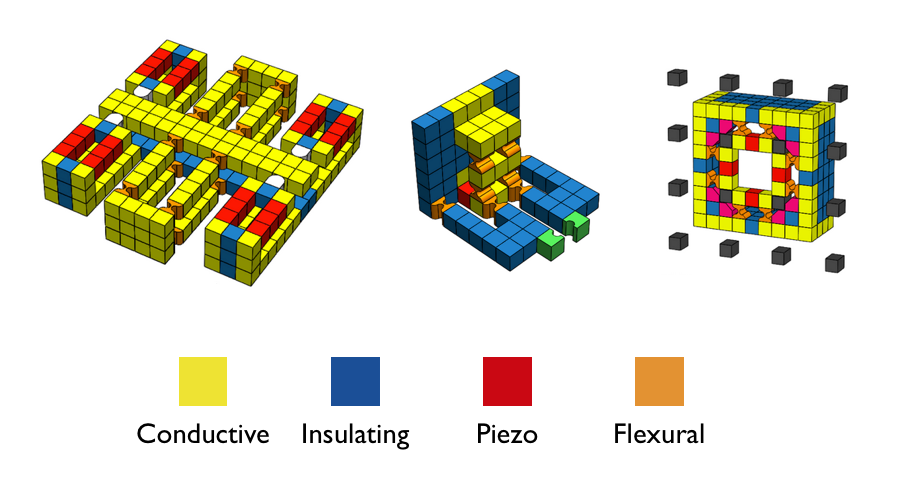
\includegraphics[width=\linewidth]{willMockups.png}
  \caption{Design mock-ups of assembler components made from digital materials by Will Langford.  From left to right: a linear actuator, a part gripping mechanism, a clamping mechanism.  None of these designs has been evaluated in simulation.}
  \label{fig:willMockups}
\end{figure}
The nano-assembly I've described will look very different from the way we make things today, and opposes many of the assumptions baked into traditional Computer Aided Design (CAD),  Computer Aided Manufacturing (CAM), and robotics.  This assembly strategy follows from an existing line of research called "digital assembly", where discrete parts are assembled on a regular, periodic lattice.  Mechanical systems are built with discrete modules of rigid and flexural components, and electronics and controls are distributed spatially across a machine (Fig \ref{fig:willMockups}).  Large structures appear to be "living" in the sense that their surface is teeming with nano-robots, detecting and correcting errors and performing other functions.  The environment is highly structured, allowing locomotion systems to position themselves globally by counting local movements across a lattice.  Machines receive instructions from their environment to coordinate various tasks.
\\

\section{Proposed Work}

I propose to build a design/simulation environment for digital materials based on realistic materials and physics, so that structures designed within this virtual environment may be physically realized one day.  I will use this virtual sandbox to design basic functional elements needed for the eventual goal of building a physically realizable assembler capable of self-replication.  Some elements of interest include mechanisms for grasping and moving parts in the assembler's environment, locomotion systems, information storage and retrieval, amplification, and digital logic.

\subsection{Part Types}

A major part of the initial phase of this project involves a literature review of research spanning biology, cellular automata, modular robotics, and materials science to pick the basis set of parts, their length scale, and a scheme for joining them together.  Initial sketches of the part types include rigid, flexure, piezo, conductive, insulating, capacitive, and resistive and scales ranging from $\mu$M to mm on a side.  The parts may become more complex for larger scales of bricks (transistors/logic gates).

\subsection{CAD Interface}

%\begin{figure}
%  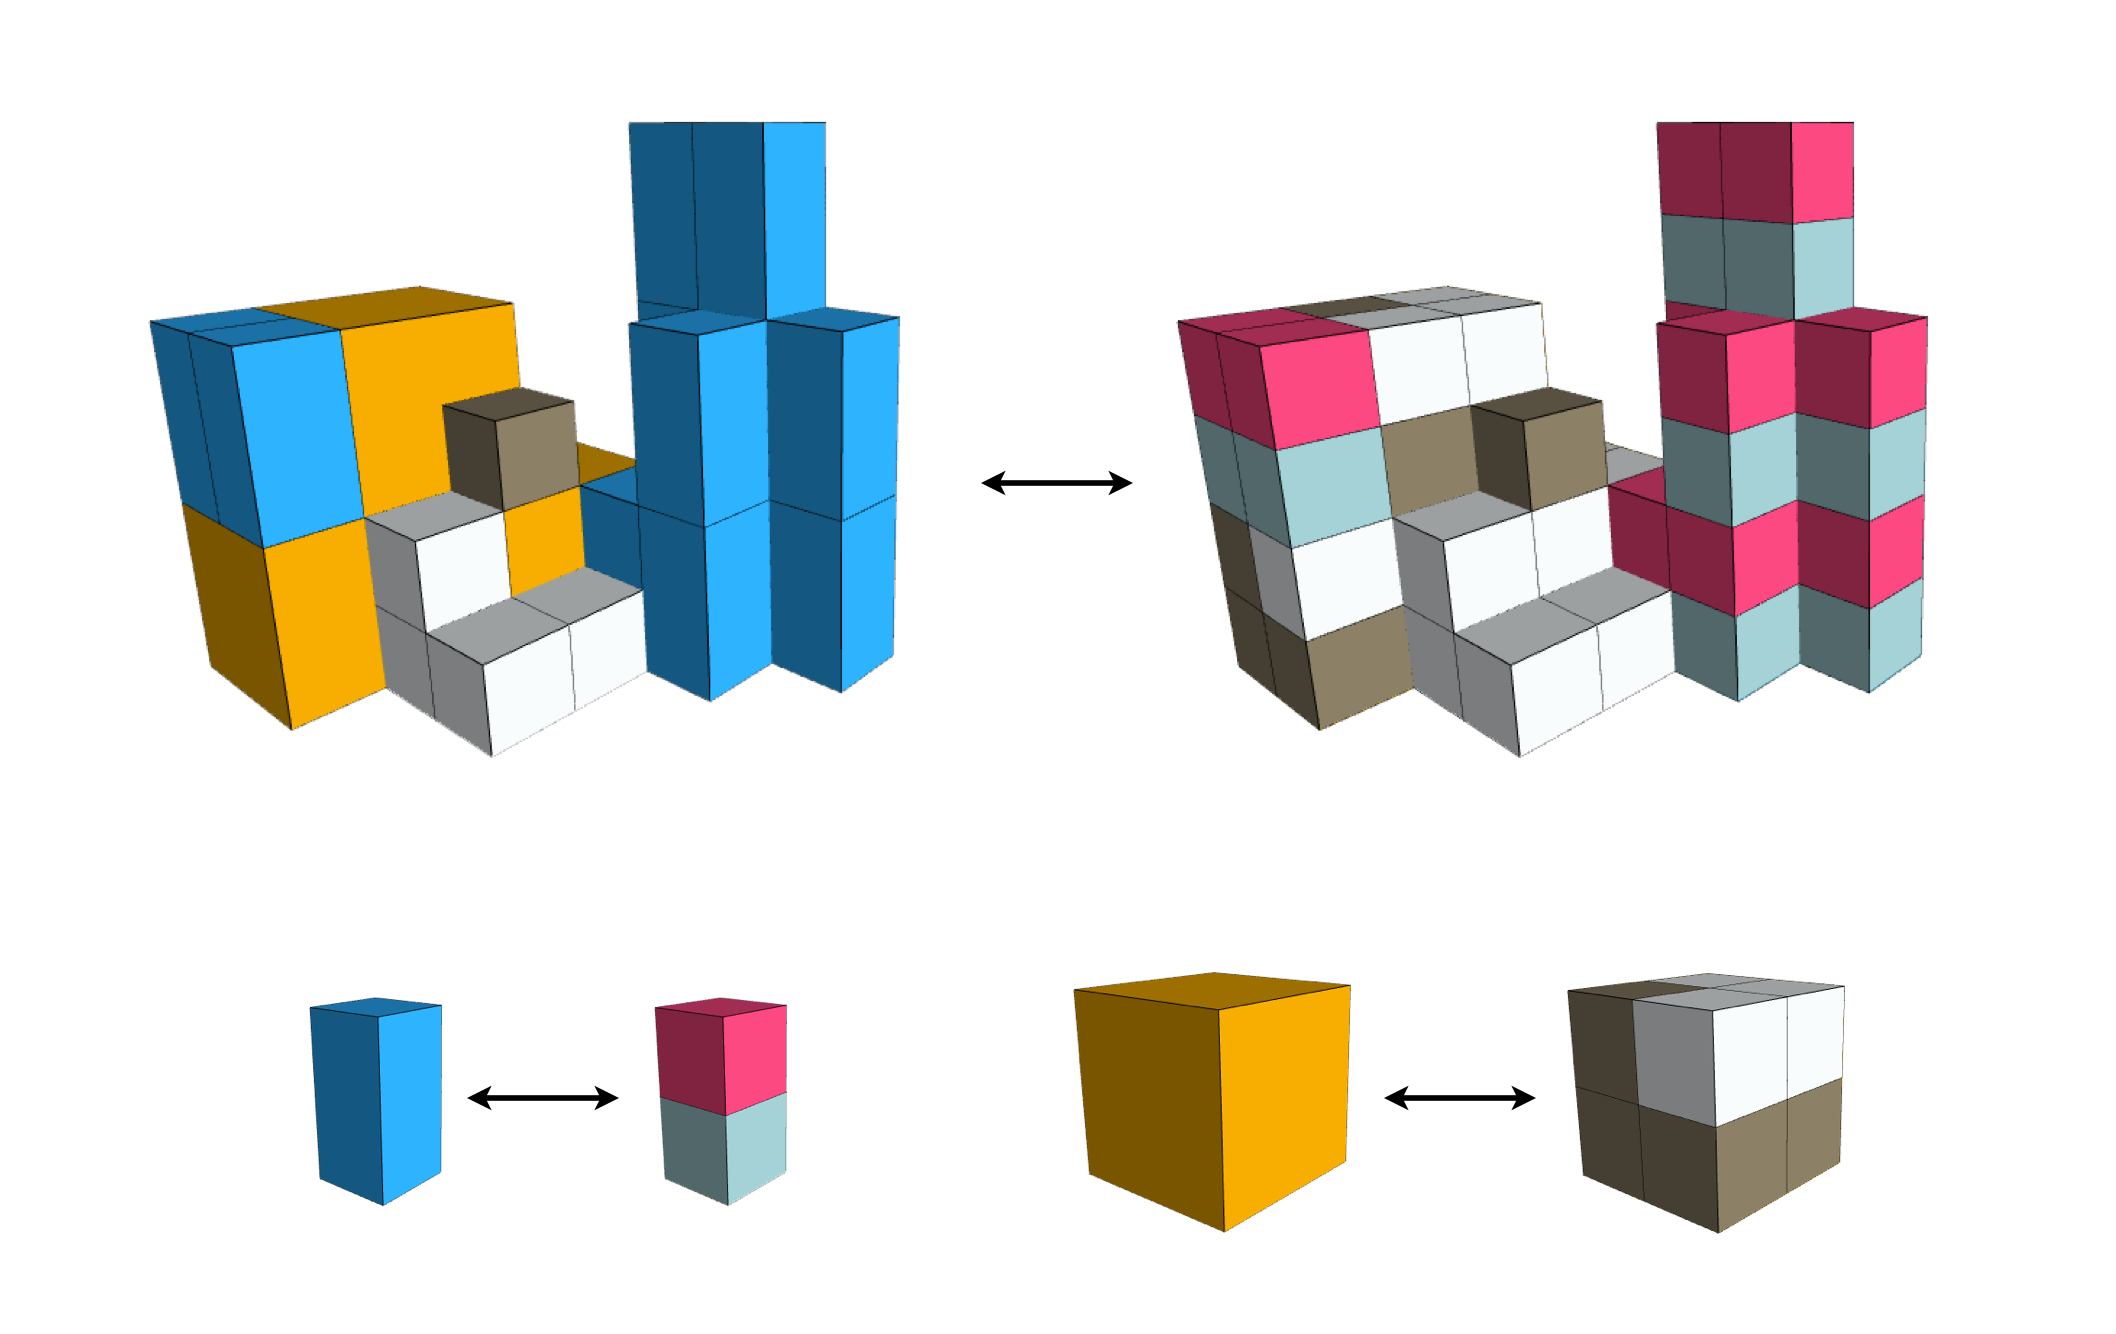
\includegraphics[width=\linewidth]{hierarchicalDecomp.png}
%  \caption{Hierarchical decomposition of lattice assembly. All hierarchical components are parametrically linked to a hierarchical material definition.}
%  \label{fig:hierarchicalDecomp}
%\end{figure}

Borrowing some classes and frameworks I've started in DMDesign, I will create a new project for the work spawned from this thesis.  All geometry will be assumed to fit on a regular cubic lattice, though flexural deformations may allow for off-grid motions.  Geometry will be represented in a hierarchical fashion (as is the case in DMDesign), where subassemblies of parts can be defined and patterned across a design, and all instances of a subassembly are linked parametrically to the same definition.

%\begin{figure}
%  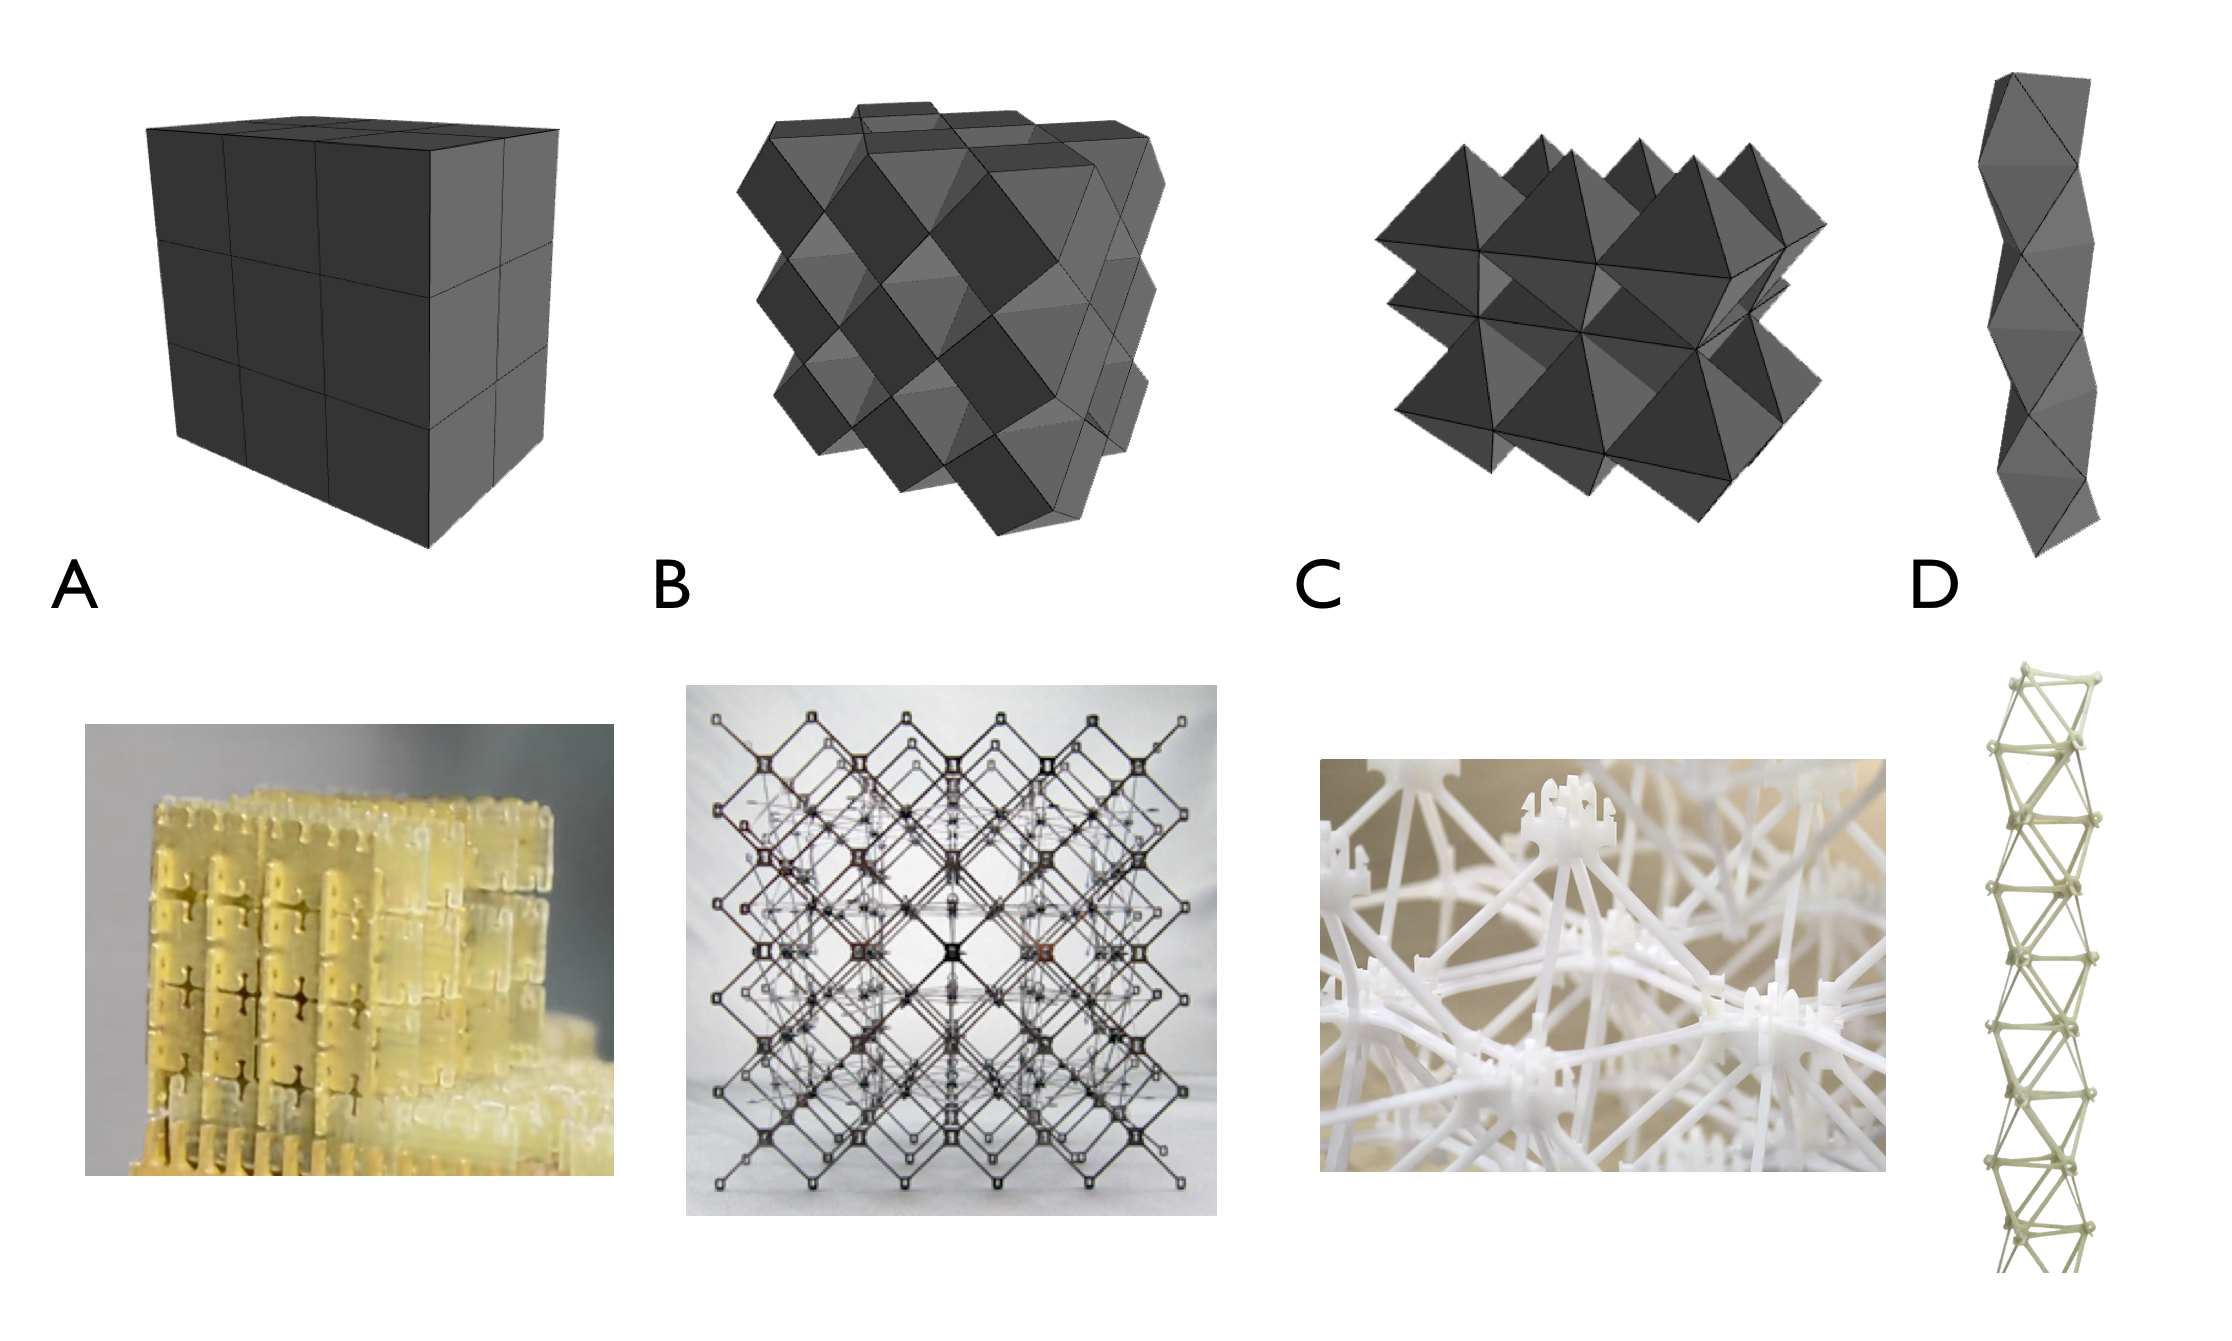
\includegraphics[width=\linewidth]{latticeVirtualRealComp.png}
%  \caption{Comparison of virtual lattice types with their real world counterparts.}
%  \label{fig: latticeVirtualRealComp}
%\end{figure}

%\begin{figure}
%  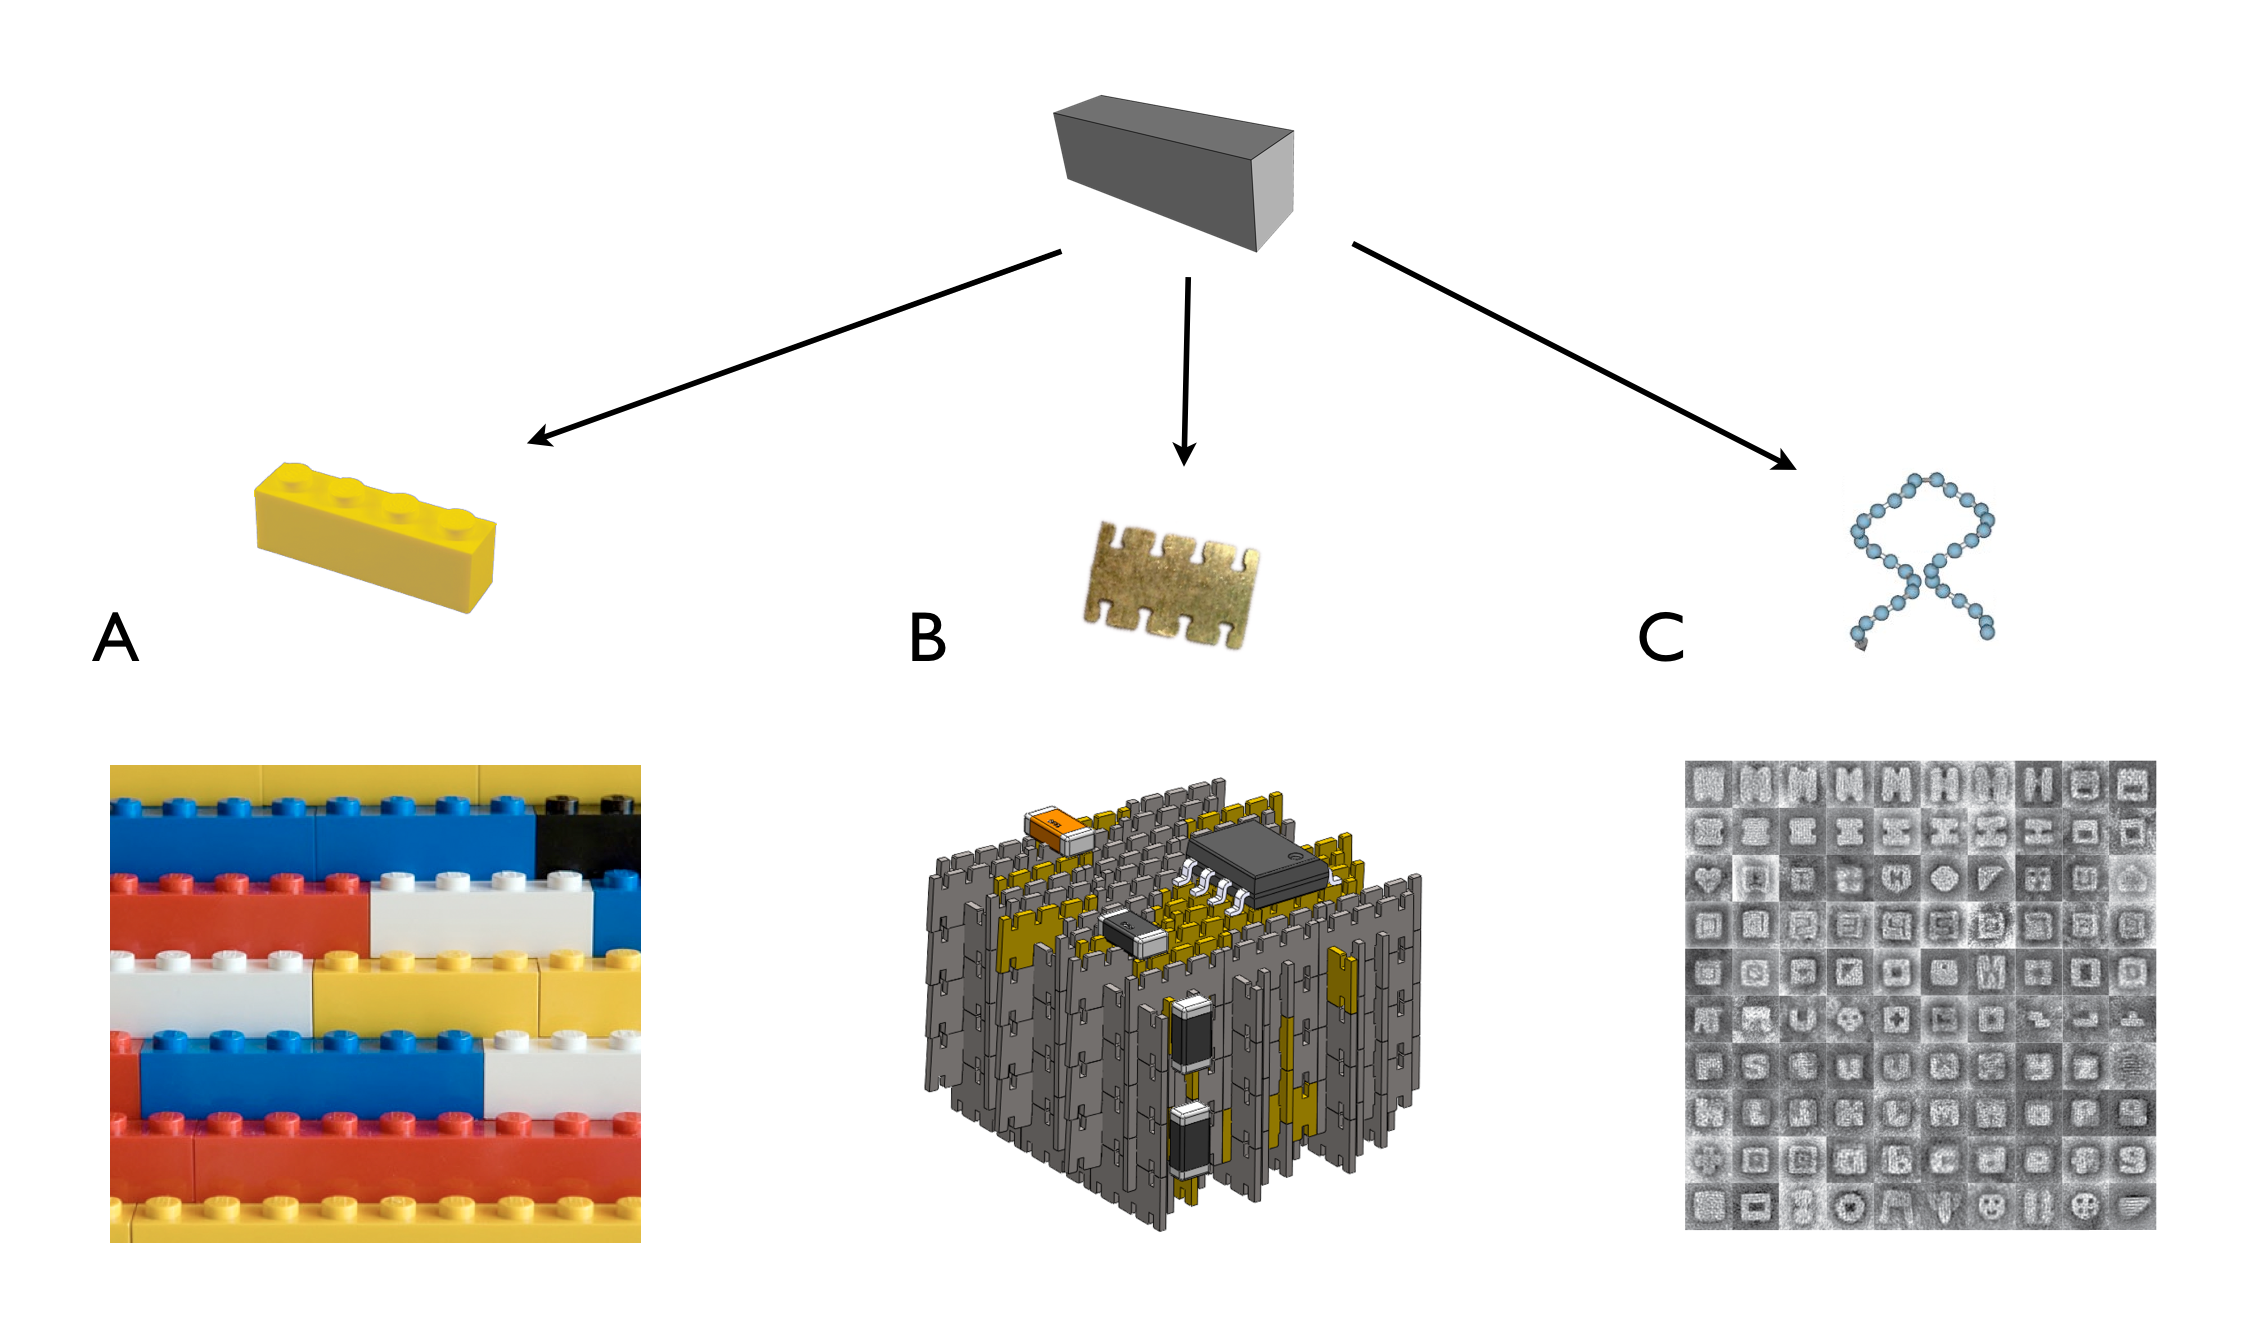
\includegraphics[width=\linewidth]{partAbstraction.png}
%  \caption{Part abstraction from lattice primitive.}
%  \label{fig: partAbstraction}
%\end{figure}

\subsection{Simulation Engine}

Dynamic simulation occurs at the granularity of the cell by modeling only local interactions between a cell and its immediate neighbors.  This way, as an assembly is designed through the CAD interface, its corresponding simulation model is constructed at the same time.  I hope that by implementing a local-only mode of simulation, I will be able to reuse the same connectivity model for both mechanical and electronic simulation, and cut down on computational costs.
\\

Locating parts on regularly spaced intervals on a lattice allows for computational shortcuts in simulation.  Depending on the nature of the mechanical and electronic simulation, I may be able to use a hash table to increase performance\cite{Gosper1984}, especially for repeating hierarchical structures within a model.  Previous work has adapted the hashlife algorithm for kinematic systems of cellular automata\cite{Stevens2010}.  I will surely need to spend some more time looking into this literature before implementing it in my own system.
\\

Additionally, I will need to implement some kind of collision detection for this system.  Due to the prevalence of gaming, there are an assortment of published algorithms to speed up  collision detection over the obvious naive approaches.  Many physics engines rely on a boundary representation of an object to detect collision with other boundaries - if objects are moving too quickly this can lead to unexpected results.  The voxels in my geometry will together define a volume of space, and the cells forming the boundary of this volume are known; I will leverage this to cut down the computational costs of collision modeling in my simulations.

\subsection{Approach}

The proposed digital materials sandbox will be built in Javascript using the following dependencies (more may be added):
\begin{itemize}
\setlength\itemsep{0em}
\item \href{http://threejs.org/}{Three.js} is a library that makes WebGL easy to use without sacrificing much in performance
\item \href{http://requirejs.org/}{RequireJS} is a framework for asynchronously loading javascript modules and dependencies
\item \href{http://backbonejs.org/}{Backbone.js} is a framework for managing UI events and giving structure to an interactive application
\item \href{https://jquery.com/}{JQuery} is a library that simplifies interactions with HTML and helps maintain cross-browser support
\item \href{http://underscorejs.org/}{Underscore} is a library with lots of useful functions for dealing with arrays and javascript objects
\end{itemize}

I know I will take some performance hit writing this application in JavaScript as opposed to a strongly-typed language like C running natively, but for this first implementation it makes sense to do start with a programming environment that I can rapidly develop in and experiment with.  If it turns out that I need to design very large structures in CAD or performance is getting in the way, I will consider porting the codebase into a compiled format.  With some optimization of the rendering, it is possible to render 100-200k voxels on the screen at 30fps in Three.js, it is unclear at this time exactly how costly the simulation will be.
\\

Aside from my own familiarity with web development, I'm interested in using HTML5/ Javascript for this application because it allows easier access to the code than any other platform.  Though user studies are not a component of this work, there is a long history of communities of users building things in these types of sandbox environments that surpass anything the developers were able to imagine.  There is a lot of talent beyond the immediate neighborhood of CBA, and I'd like to try to make this codebase as available as possible for anyone interested in exploring this new way of making things.

%\subsection{Assembly}
%
%\begin{figure}
%  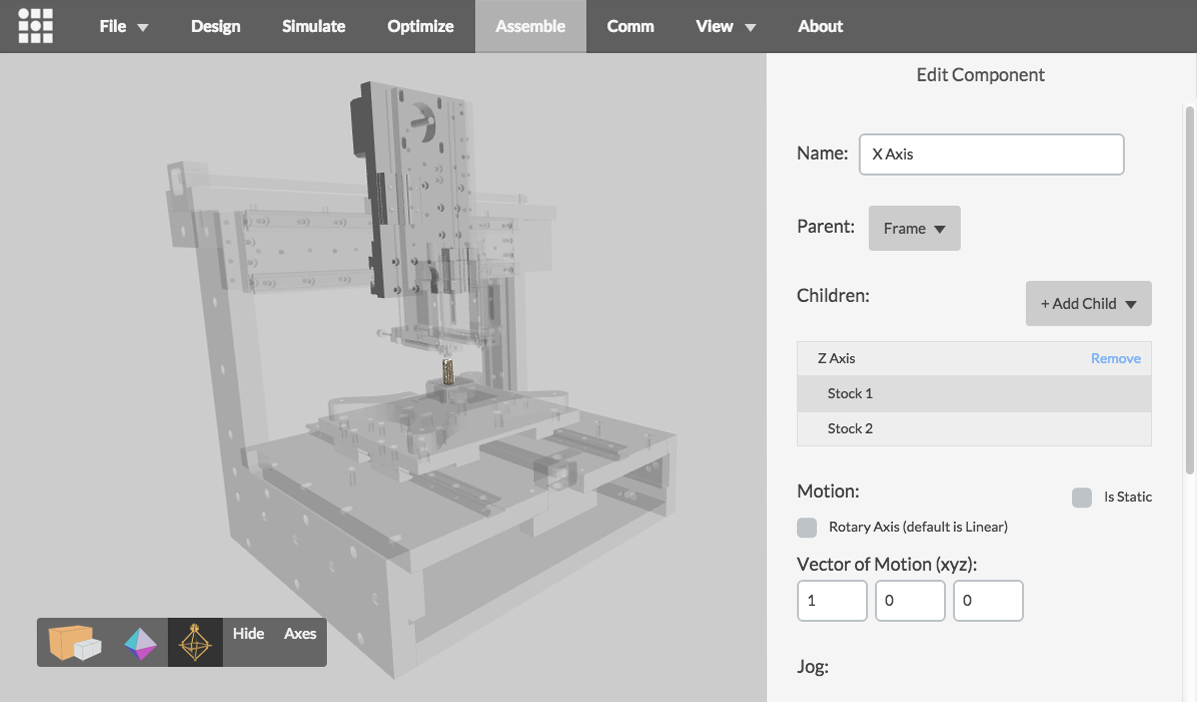
\includegraphics[width=\linewidth]{assemblerSetup1.png}
%  \caption{Screenshot of current assembler config GUI.}
%  \label{fig: assembleSetup1}
%\end{figure}
%
%\begin{figure}
%  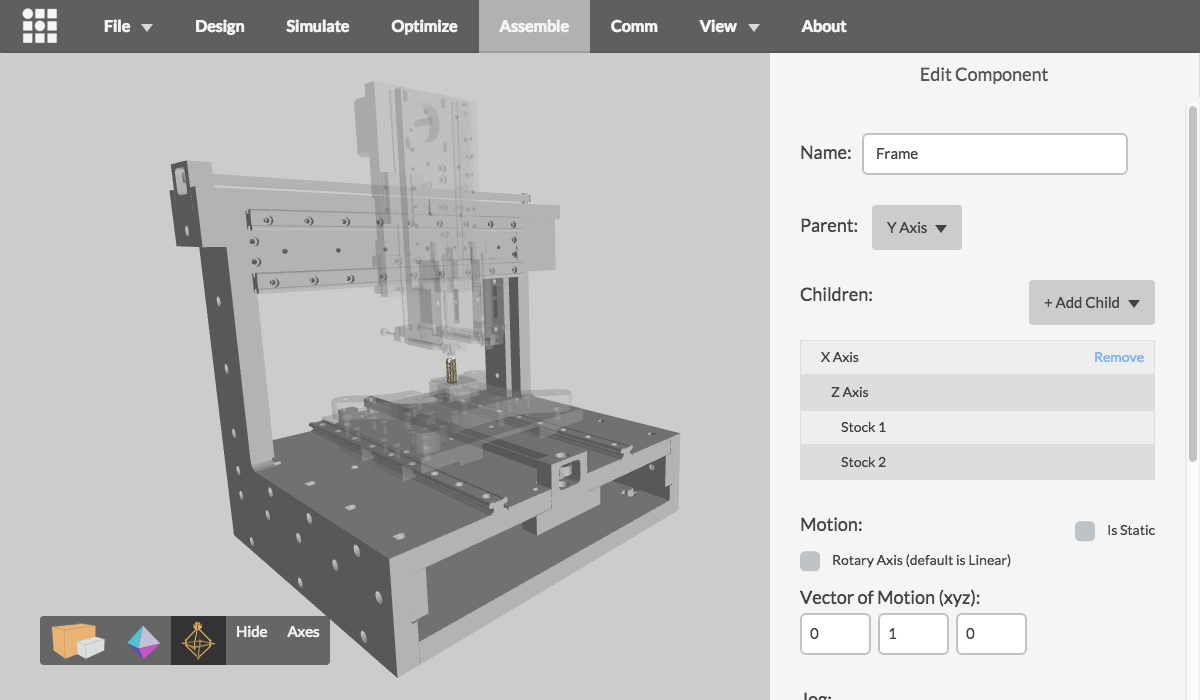
\includegraphics[width=\linewidth]{assemblerSetup2.png}
%  \caption{Screenshot of current assembler config GUI.}
%  \label{fig: assembleSetup2}
%\end{figure}
%
%urdf, tree description for abstraction
%calculate reverse kinematics
%abstraction of strategies and assemblers/low level operation

%\subsection{GUI}
%
%\begin{figure}
%  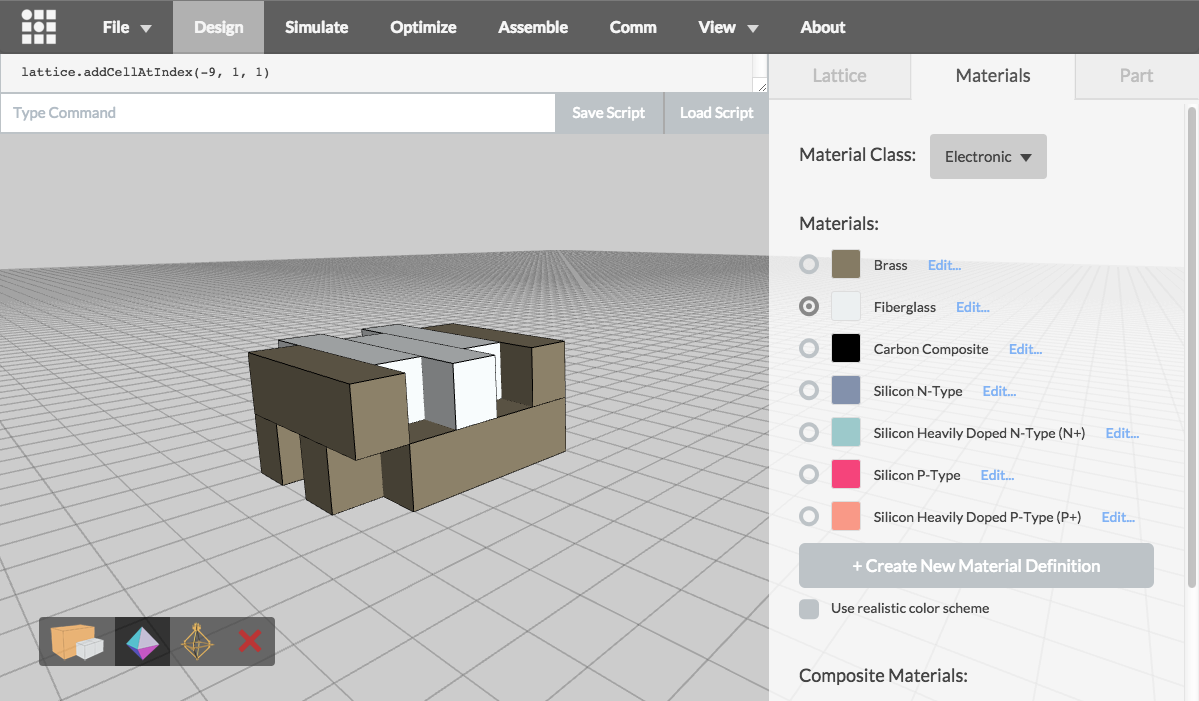
\includegraphics[width=\linewidth]{designGUI.png}
%  \caption{Screenshot of current design GUI.}
%  \label{fig: designGUI}
%\end{figure}
%
%\begin{figure}
%  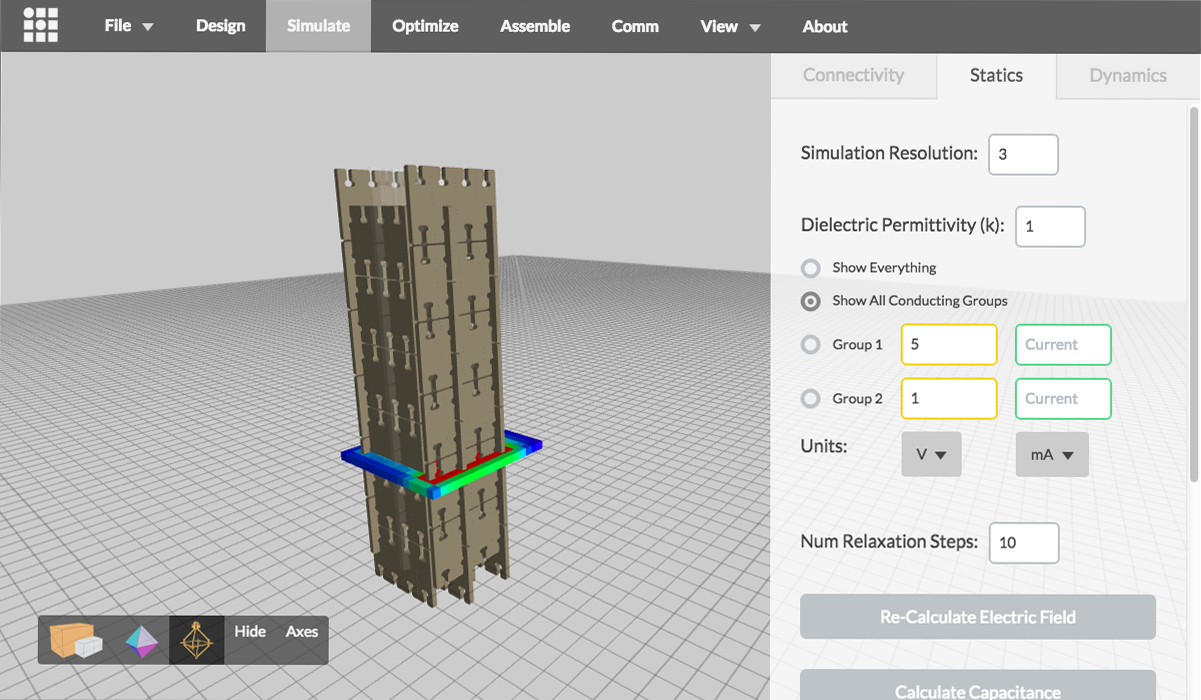
\includegraphics[width=\linewidth]{simGUI.png}
%  \caption{Screenshot of current simulation GUI.}
%  \label{fig: simGUI}
%\end{figure}
%
%\begin{figure}
%  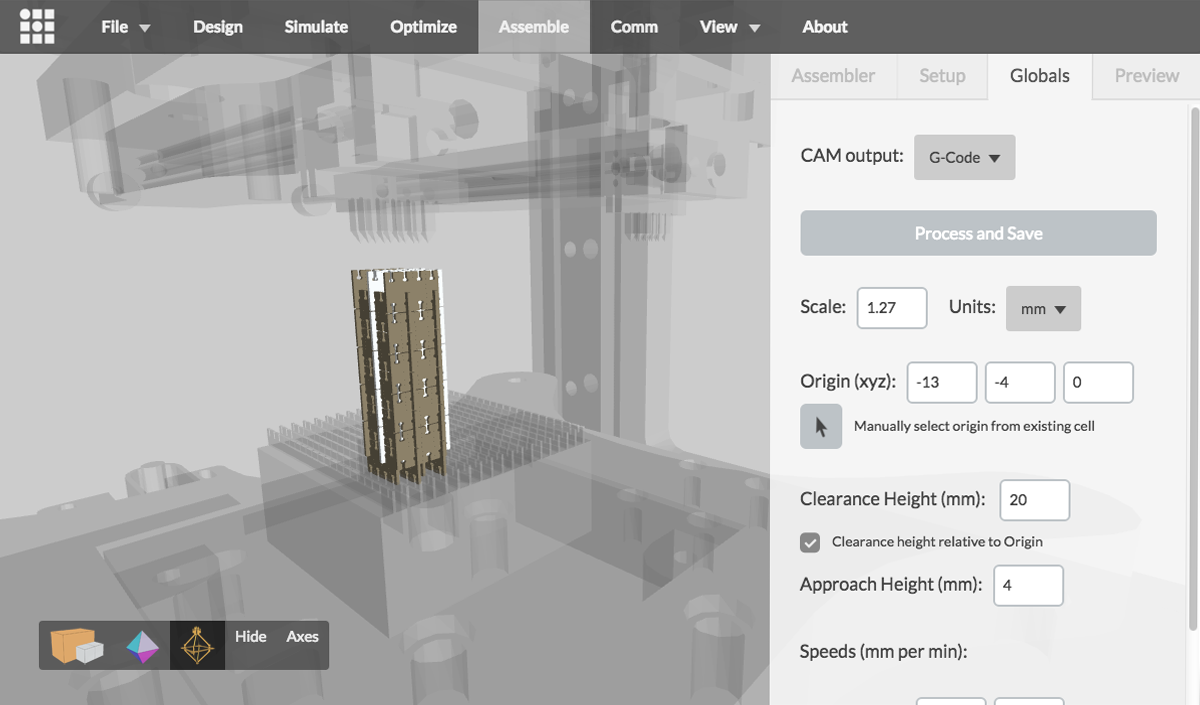
\includegraphics[width=\linewidth]{assembleGUI.png}
%  \caption{Screenshot of current assemble GUI.}
%  \label{fig: assembleGUI}
%\end{figure}
%
%javascript, etc, etc

%\subsection{API}
%
%Lattice, Cell, Material, CompositeMaterial classes.
%
%\begin{figure}
%  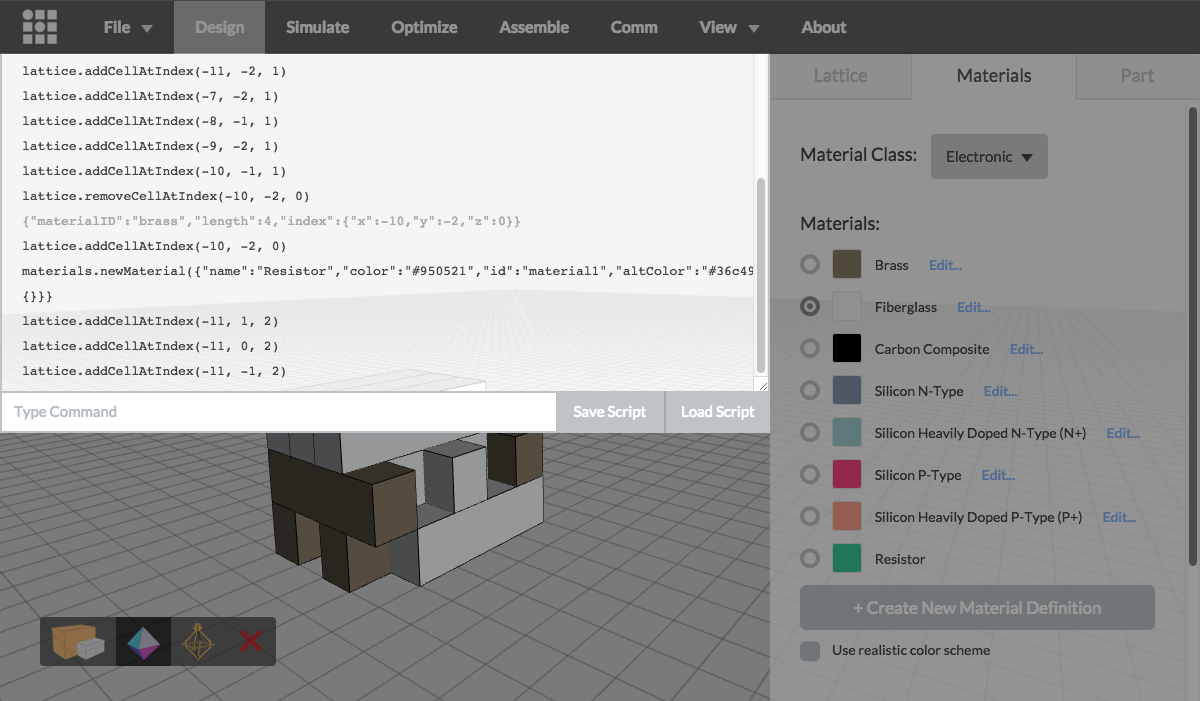
\includegraphics[width=\linewidth]{scriptGUI.png}
%  \caption{Screenshot of current script GUI for API with scripting console highlighted.}
%  \label{fig: scriptGUI}
%\end{figure}
%
%asdfdsf

\section{Contribution}

As outlined in previous sections, the main contribution of this work is to create a design/simulation environment where anyone can start to explore the rich design space around digital materials in a physically realistic way.  This work will inform future trajectories in CBA research and in the broader field of programmable materials, modular robotics, and digital fabrication.  This work is not intended to result in a manual outlining all the necessary components for self-replication based on current technology, but rather as an sandbox for exploring self-assembling systems based on the foundations of engineering and materials science rather than biology.

\section{Evaluation}

Once the CAD/simulation environment is set up, I will design several functional objects within it and evaluate their function both quantitatively and qualitatively.  Some objects that would be especially interesting include:
\begin{description}
\setlength\itemsep{0em}
\item[] locomotion systems
\item[] end effectors (gripping mechanisms, part manipulation)
\item[] information storage and retrieval
\item[] amplification of motion and signals
\item[] digital logic
\end{description}
Qualitative assessment includes evaluation of success or failure of the intended function (can a gripping mechanism grip a part), and quantitative assessment includes calculations of performance (gripping strength, speed of locomotion, volume required to implement various types of digital logic, speed of memory access, etc).

\section{Resources Required}

The majority of the work involved in this thesis will happen in the computer and require no material resources.  If required, I will use CBA's cluster for highly parallel computational operations.  Fabrication of assemblers and parts to be used in the digital assembler workflows should be considered outside the scope of material resources required by this thesis, and will be supplied by CBA.

\section{Schedule}

\begin{description}
  \item[11/6/15]\tabto{1.5cm}Proposal Due
  \item[11/9/15]\tabto{1.5cm}Crit Day Presentation
  \item[11/15]\tabto{1.5cm}Design and assembly workflow for digital materials is in a working state.  I will use elements of the classes and framework developed in that project to begin a new project specifically for the completion of the thesis.  This new project will only be concerned with the design and simulation of multimaterial assemblies on a cubic lattice (for simplicity).  Finish CAD interface.
  \item[12/15]\tabto{1.5cm}Hello world of basic CA behind the electronic/mechanical simulation.  Not worrying about efficiency at this point, get cells moving and communicating.  Start making decisions about scale and part types, num materials, geometry, allowed interactions, interfaces.
  \item[1/15]\tabto{1.5cm}Build out main components of simulation engine.
  \item[2/15]\tabto{1.5cm}Collision detection strategies, unconnected modules should be able to interact with each other
  \item[3/15]\tabto{1.5cm}Refinement and optimization of simulation engine
  \item[4/15]\tabto{1.5cm}Performance optimization and design studies
  \item[5/15]\tabto{1.5cm}Design studies and writeup
  \item[6/6]\tabto{1.5cm}Thesis Due
\end{description}

}

%% This is an example first chapter.  You should put chapter/appendix that you
%% write into a separate file, and add a line \include{yourfilename} to
%% main.tex, where `yourfilename.tex' is the name of the chapter/appendix file.
%% You can process specific files by typing their names in at the 
%% \files=
%% prompt when you run the file main.tex through LaTeX.

\singlespacing{

\chapter{Related Work}


The following sections outline current research into digital assembly across scales, CAD/simulation packages which occupy a similar space to what I propose, and programmable self assembly.

%An active area of synthetic biology explores the possibility of creating a viable cell from scratch based on knowledge about the core systems required for metabolism, cell maintainance, and self replication\cite{Forster2006}.  To date, efforts at creating this "minimal cell" have only been successful using a top down approach - starting with an organism with a minimal genome and reducing its genes further\cite{Glass2006}\cite{Gibson2010}.

\section{Digital Assembly}

Digital assembly is an emerging multimaterial fabrication technique where a finite set of discrete part types are (often reversibly) joined to form larger structures in a regular lattice.  Programmable functional behavior is achieved by patterning parts with different material properties across an assembly.  In the macro scale, the assembly process is orchestrated by one or many robotic assemblers.  Self-alignment features and the regular spacing of the parts help to minimize the complexity of a robotic assembler, and maintain global metrology through local interactions.  At nano scales, assembly is guided by programmable self-assembly mechanisms.


\subsection{Macro Assembly}

Cheung showed that carbon fiber composite parts can be reversibly assembled to form ultralight materials for aerospace applications\cite{Cheung2013}.  Programmable flexibility is achieved by pattering rigid and flexural parts across an assembly and also by varying the density and connectivity of the parts.  Additional research into digital assembly of structural elements is ongoing at CBA, including modeling of the parts and assemblies using finite element analysis\cite{Calisch2014} and designing new part geometries and robotic assemblers\cite{Carney2015}.

\subsection{Micro Assembly}

\begin{figure}
  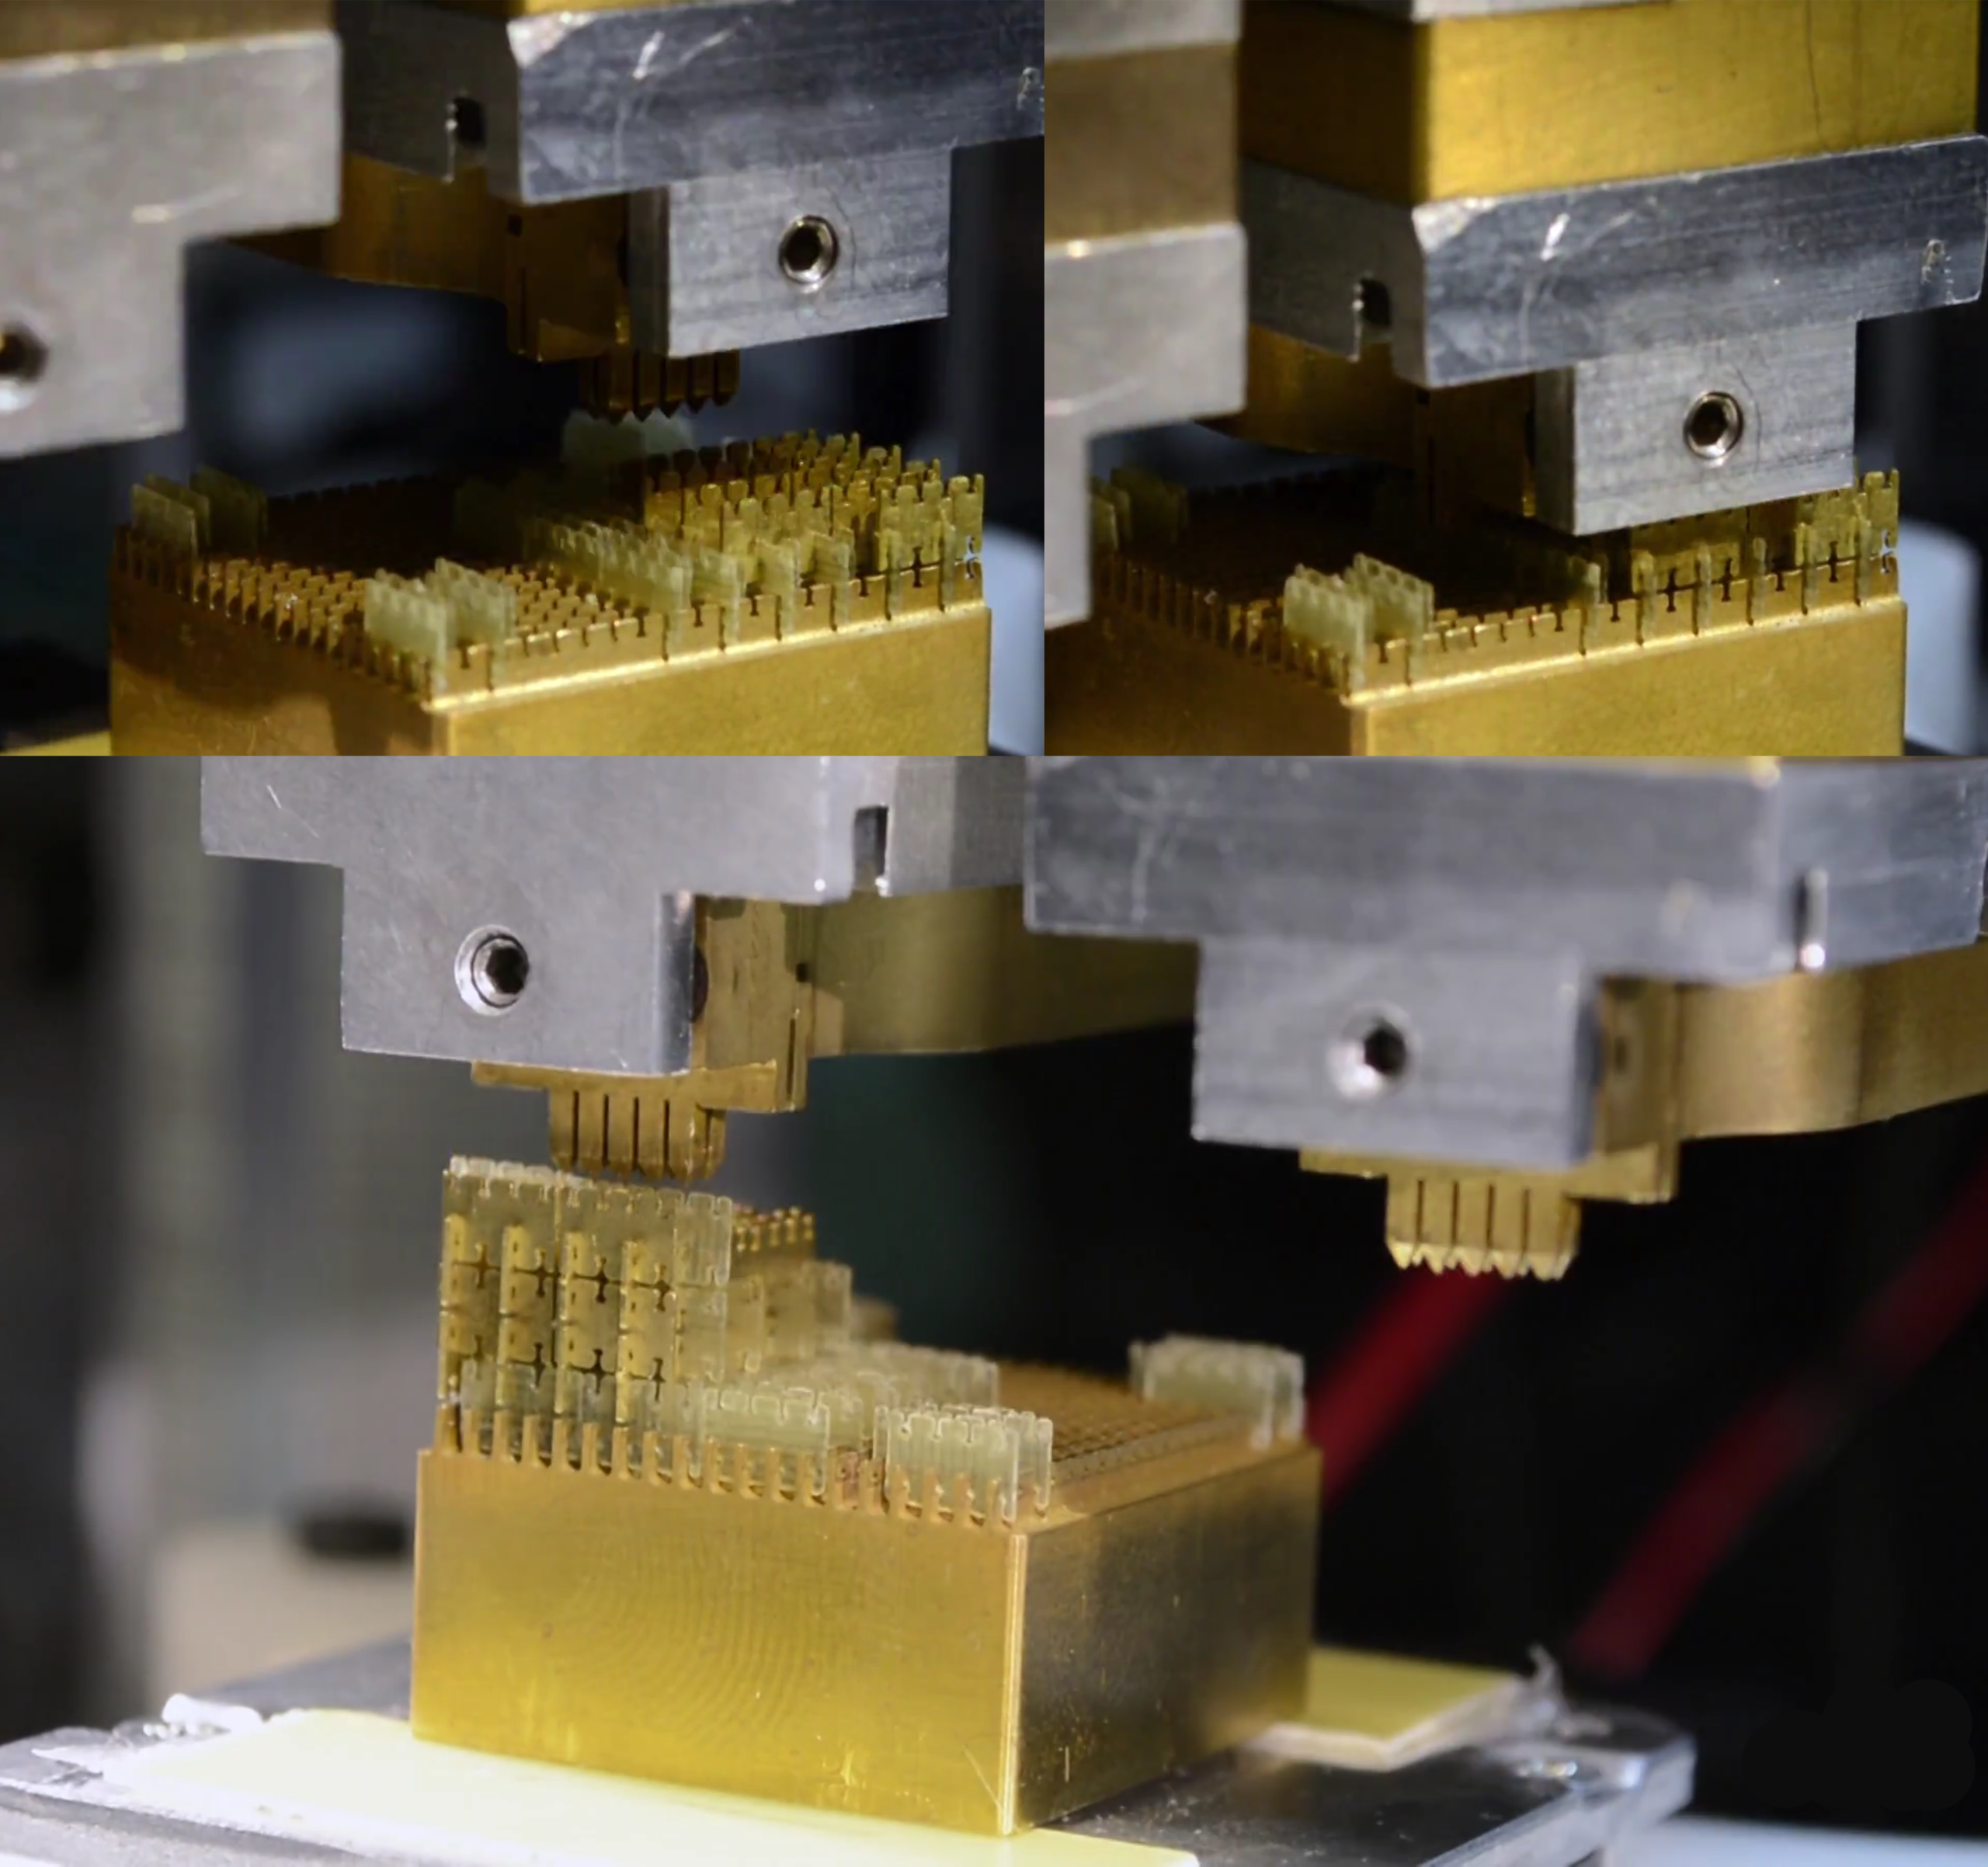
\includegraphics[width=\linewidth]{willAssembler.png}
  \caption{"Stapler" assembler designed by Will Langford assembles conductive and insulating discrete part types to form electronic structures with tunable capacitance and inductance.  \textit{Image Credit: Will Langford 2015}}
  \label{fig:willAssembler}
\end{figure}


%\begin{figure}
%  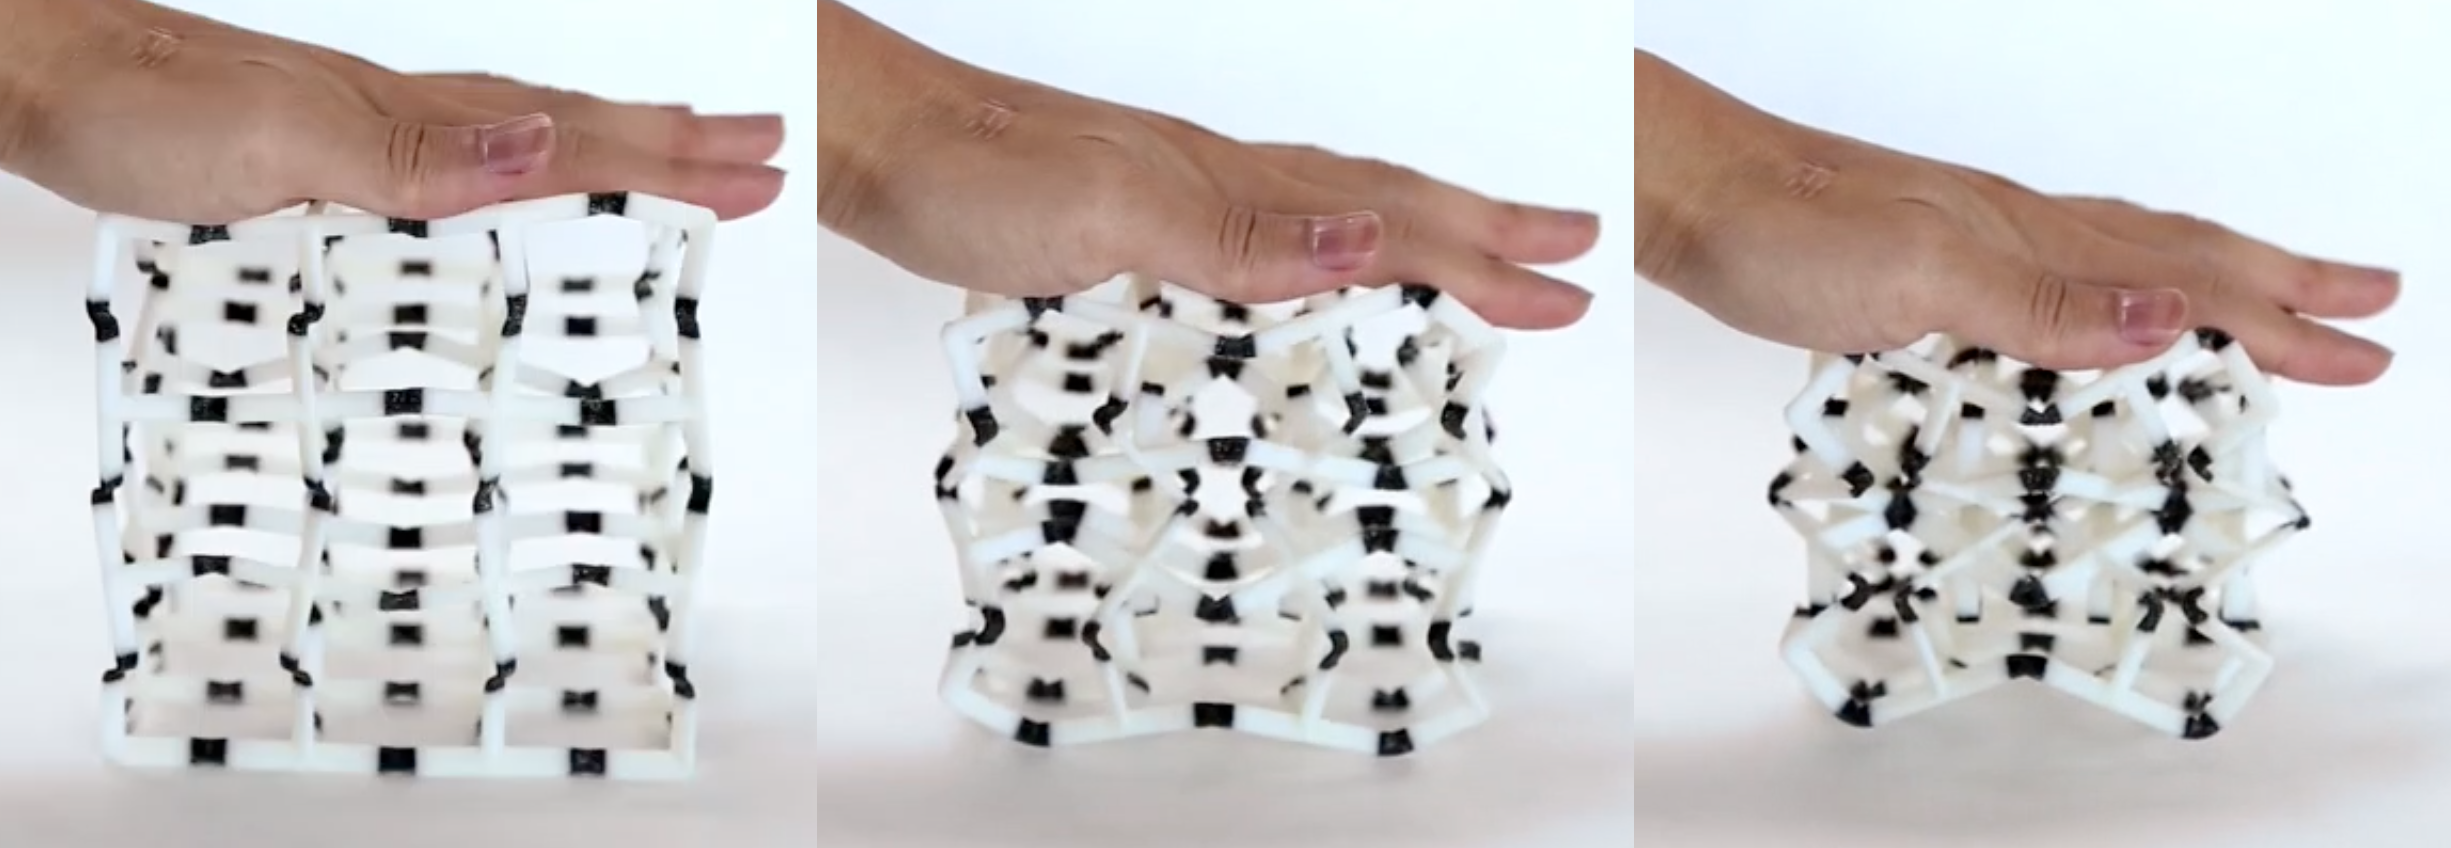
\includegraphics[width=\linewidth]{objetMultimaterial.png}
%  \caption{Mechanical properties programmed by material deposition in Objet 3D print.}
%  \label{fig: objetMultimaterial}
%\end{figure}

Langford demonstrated how conducting, insulating, and resistive part types ranging in scale from mm-$\mu$m could be assembled to form any passive electronic component, including antennas and matching networks\cite{Langford2014}.  Langford designed and built a dual-material assembler (Fig: \ref{fig:willAssembler}) for constructing passive electronic structures from conducting and insulating parts (\href{http://dma.cba.mit.edu/stapler/video/dualstapler_full_1.mp4}{video})\cite{LangfordWillGhassaeiAmandaGershenfeld2016}.  Langford suggests that by extending the part types to include several types of silicon components, discretely-assembled active components like diodes and transistors would be possible.  Work toward the fabrication and realization of these silicon components is ongoing.  This work follows from previous work by Popescu et al. on reversibly assembled "GIK" structures spanning many length scales and material types\cite{Popescu} and also work by Ward on discretely assembled electronics\cite{Ward2010}.
\\

Hiller et al. propose a method of additive manufacturing using multimaterial voxel building blocks\cite{Hiller2009a}.  They explore various voxel decompositions of 3D geometry and assess their suitability for rapid, parallel assembly processes (\href{https://www.youtube.com/watch?v=-szjlhVMGh4}{video}).  Possible applications discussed include desktop manufacturing, especially for electromechanical and microfluidic devices.  Hiller et al. also propose reversible processes for disassembling a voxel assembly back into its constituent parts\cite{Hiller2005}.
\\

Though not a reversible process, multimaterial 3D printing (most notably by the Objet printer) deposits material in voxels on the order of ~10$\mu$m$^{3}$ with a total build volume on the order of 1x10$^{10}$ voxels\cite{Objet1000}.  Multimaterial 3d printing has been demonstrated in optical\cite{Willis2012}, electronic\cite{Ahn2009}, and structural applications\cite{Skouras2013}\cite{Schumacher}\cite{Bacher2014}.

\subsection{Nano Assembly}

DNA bricks is a system of discrete assembly based on complementary base pair interactions of short segments of DNA\cite{Ke2012}; DNA bricks is a branch of a field called DNA origami\cite{Rothemund2006} or DNA computing\cite{Seeman1982}\cite{Adleman1994}.  The brick assemblies have a spatial resolution of 2.5nm and the longest dimension of a DNA brick assembly measures on the order of 1$\mu$M\cite{Ke2014}.  Unlike the previously discusses processes, DNA bricks assembly takes place through passive, stochastic interactions between DNA strands in solution, rather than guided assembly by robotic assemblers.
\\

CBA is actively involved in the design of nano-manipulation devices and work toward scaling down the micro-electronic parts designed by Langford\cite{Langford2014} into the nanoscale.

\section{Dynamic Simulation Techniques}

\subsection{Dynamic Simulation of Elastic Solids}

A large portion of the work involved in this thesis involves the development of a dynamic simulation engine for elastically deformable solids.  \href{https://en.wikipedia.org/wiki/Solid_mechanics}{Solid mechanics} is the study of the motion and deformation of solid bodies under external forces, changes in temperature, and other stresses.  Solid mechanics differentiates itself from other branches of continuum mechanics because solids are assumed to have a preferred rest shape.  This thesis is concerned with a subset of solid mechanics called elasticity, where materials return to their initial rest shape after all external forces are removed.  A more complete discussion of solid mechanics is given in Bower\cite{Bower2009}.\\  

This thesis explores both isotropic and anisotropic materials.  A material is isotropic if it responds the same to an external force no matter its orientation; materials comprised of oriented fibers or other directional structures typical display anisotropic behaviors.  

\subsubsection{Simulation Techniques for Solids}


FEA vs Mass-Spring vs CA\\
few works well for linear - non linear for large deformations may require remeshing\\
mass spring methods - widely used in computer graphics, better for large deformations and non linear, less accurate\\
differential elements\\
lattice gas\\

\subsubsection{Numerical Integration Techniques}

Runge-Kutta\\
Euler Integration\\

\subsection{Cellular Automata}

A \href{https://en.wikipedia.org/wiki/Cellular_automaton}{cellular automaton} (CA) is a discretized model used to describe the dynamics of a system.  CAs are discrete in both space in time, meaning space is divided up into many identical "cells" and time moves forward in discrete "steps".  Each cell owns one or many state variables, which may hold binary or continuous data.  
The governing equations of a CA system are codified in the "ruleset" that applies universally across all cells in the system; typically a ruleset describes local interactions of a cell with its neighbors.  For example, in the popular CA \href{https://en.wikipedia.org/wiki/Conway's_Game_of_Life}{Conway's Game of Life}, the state of a cell in the next time step is a function of its current state and the state of its eight neighbors.\\

CAs have been used to study the requirements of self-assembling systems going back at least as early as the 1940s\cite{Neumann1966}.
Many CAs operate under extremely simple rulesets that violate basic physcial 
This by no means implies that CAs are inherently non-physical; in fact, finite difference method can be thought of as a type of cellular automata\cite{Yang2010}.
Some violations of physics found in these tools include the ability to create and destroy matter at will, actuators with infinite torque or , the absence of gravity, 


\section{CAD and Simulation Tools for Digital Assembly}

At the moment of writing this, there exist several computational tools for designing and simulating kinematic, discretely-assembled structures.

\subsection{Cellular Automata-Based Tools}

The CA-based simulation tools discussed here allow for computational efficiency at the cost of accuracy, often allowing for only quantized motions, interactions, and states.  In general, this classification of tools employs materials and mechanics that are not plausible in the real world, but are still of interest for purely computational investigations.  The earliest design and simulation tools for CA systems were a piece of graph paper or a Go board\cite{Gardner1970}.  With the introduction of personal computers and graphical user interfaces, it his now possible to compute large CA universes and study their behaviors.\\

\begin{figure}
  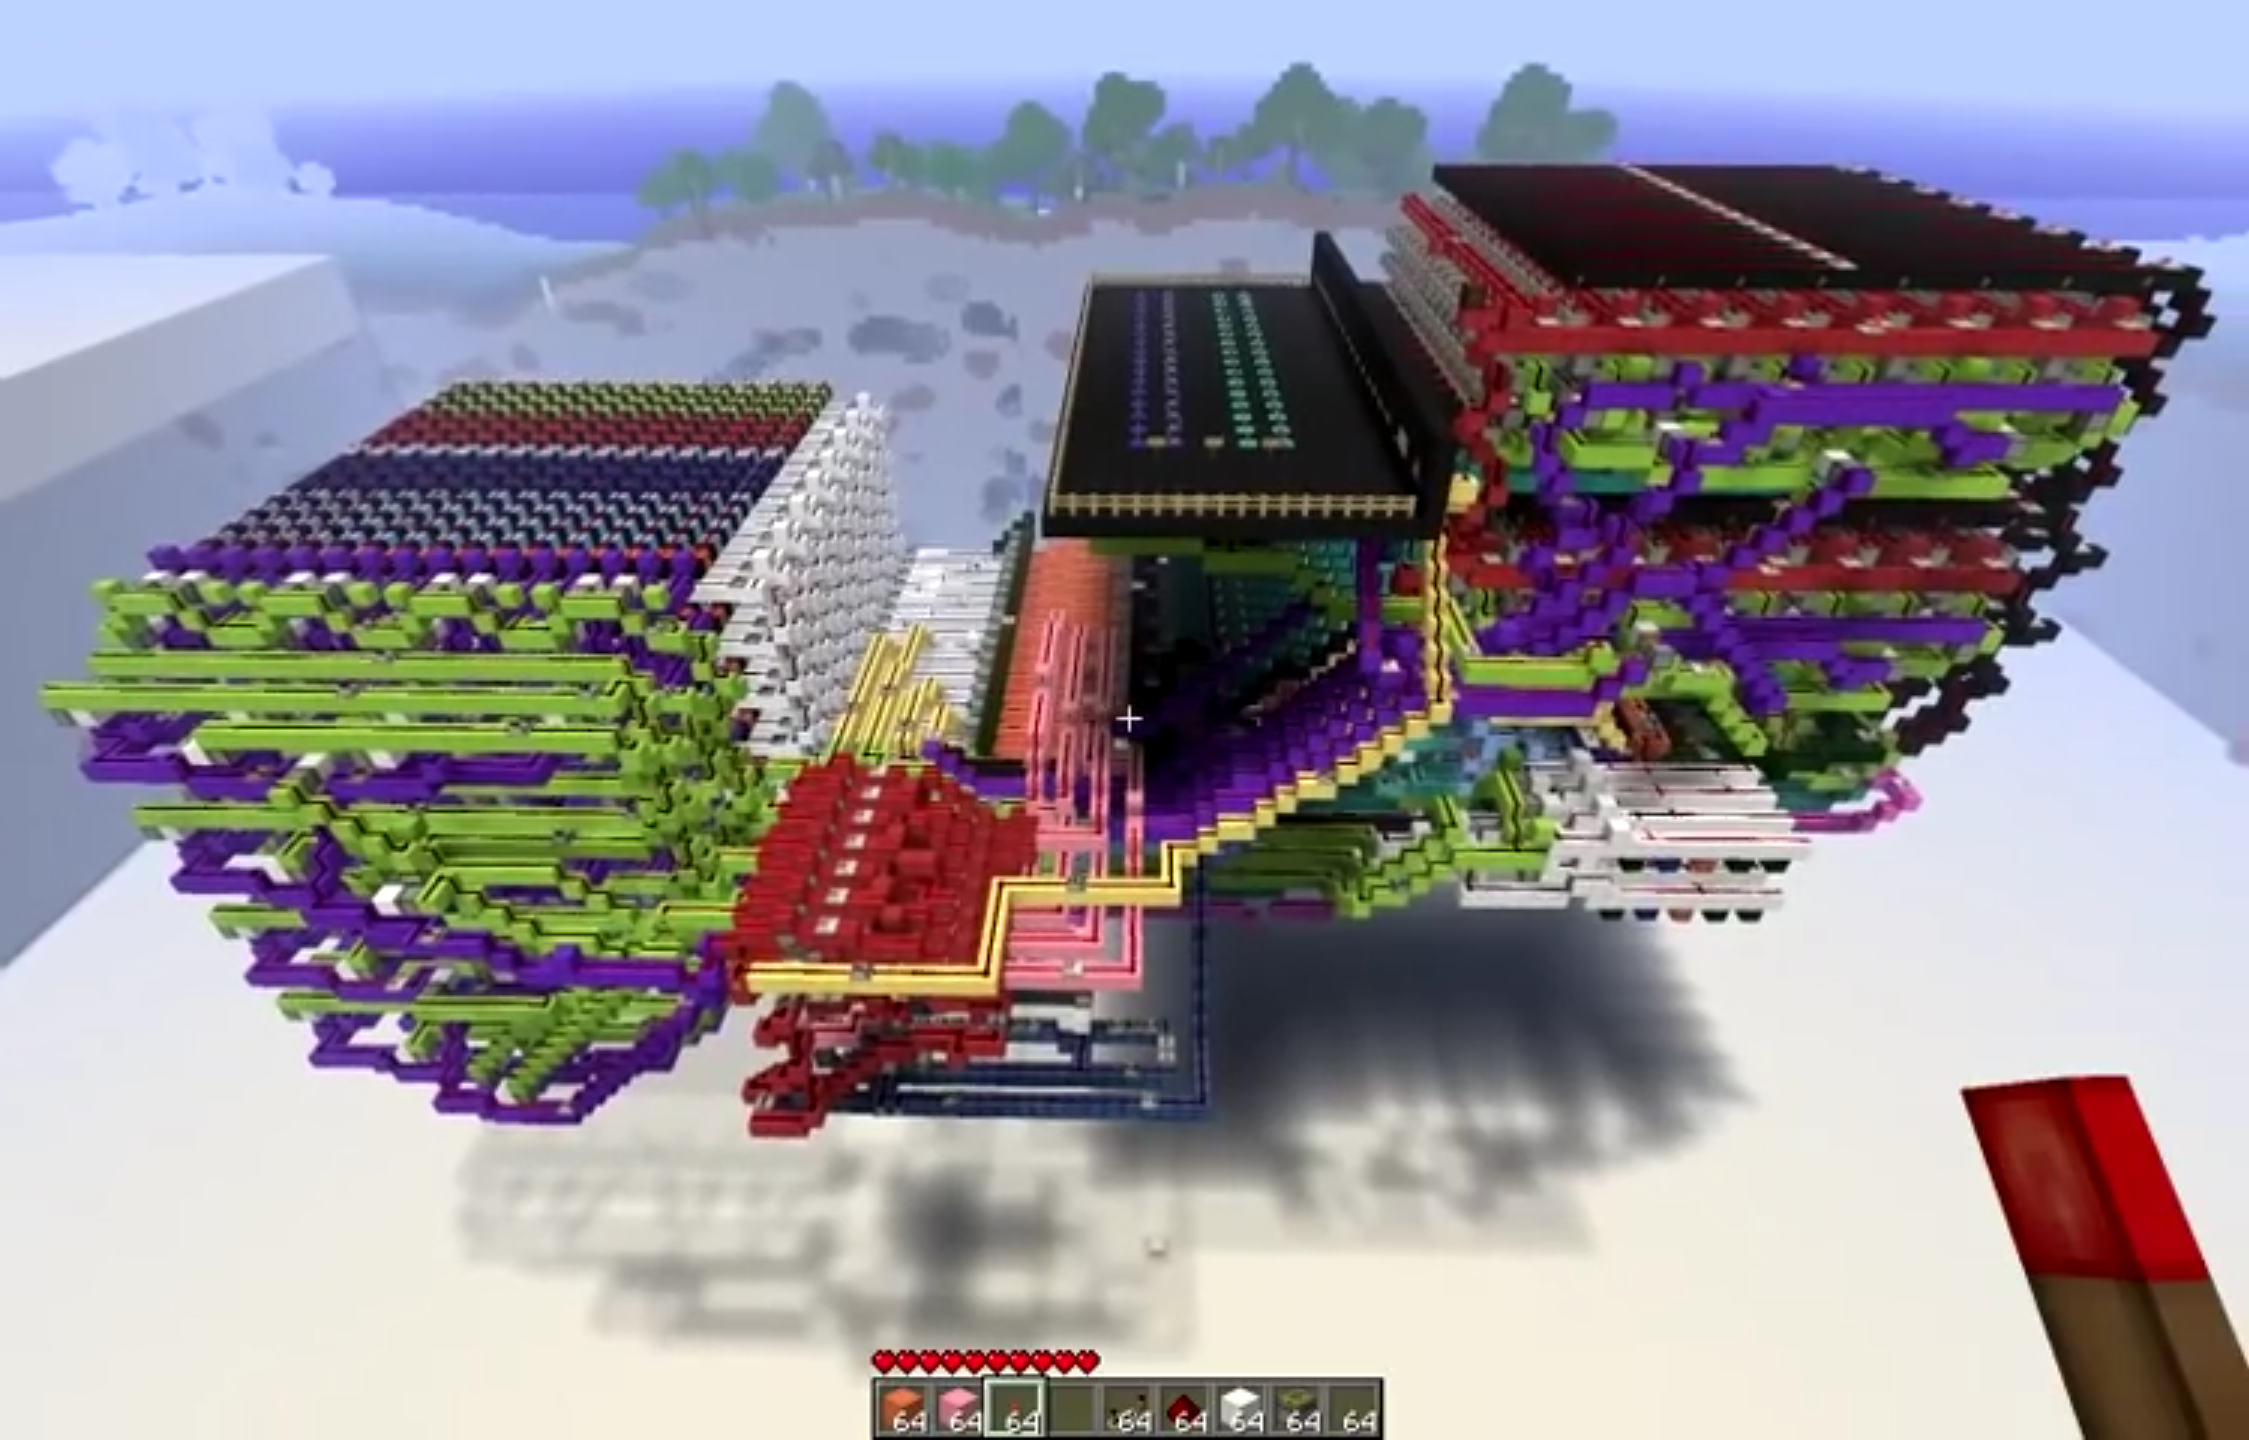
\includegraphics[width=\linewidth]{minecraft.png}
  \caption{Screenshot of a 16 bit computer built in Minecraft by user Ohm.  Full video available on \href{https://www.youtube.com/watch?v=KzrFzkb3A4o}{YouTube}. \textit{Image Credit: Ohm 2011}}
  \label{fig:minecraft}
\end{figure}
The most widely adopted example of discrete design is \href{https://minecraft.net/}{Minecraft}, a PC game that gives players the ability to construct their own worlds from over 100 different block types (Fig \ref{fig:minecraft}).  A subset of these block types form the basis of digital logic in the game and another set of part provide a means of simple 1-bit mechanical actuation\cite{MinecraftWik2016}.  Gameplay and available block types are extendable through various mods and user scripts.
\\

\href{http://golly.sourceforge.net/}{Golly} is a 2D CA simulator originally intended for Conway's game of life, but is extendable to other rulesets.  It implements Gosper's "hashlife" algorithm for optimizing the performance of the simulation\cite{Gosper1984}.  In 2010 Andrew Wade published \href{https://www.youtube.com/watch?v=A8B5MbHPlH0}{Gemini}, a self replicating machine designed in Golly using Conway's ruleset.  In 2014, Luke Shaeffer implemented a physically universal CA ruleset in Golly, based on interactions between moving particles\cite{Shaffer2014}.\\

\begin{figure}
  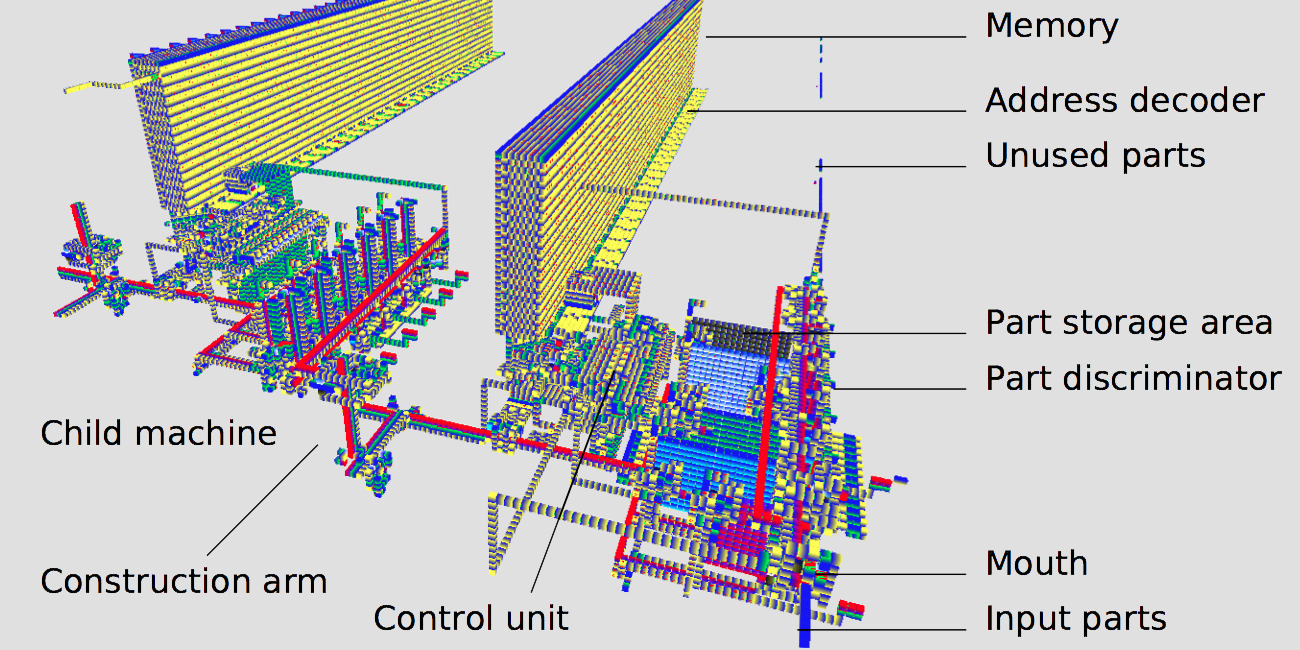
\includegraphics[width=\linewidth]{stevensConstructor.png}
  \caption{A programmable, universal constructor (shown replicating itself) built in CBlock3D by William Stevens from 5040 cells of 6 different types\cite{Stevens2009b}.  Full video of assembly process on  \href{https://www.youtube.com/watch?v=PBXO_6Jn1fs}{YouTube}. \textit{Image Credit: William Stevens 2010}}
  \label{fig:stevensConstructor}
\end{figure}
\href{https://www.youtube.com/watch?feature=player_embedded&v=PBXO_6Jn1fs}{CBlock3D} is a 3D cellular automata environment governed by logical and kinematic rules developed by William Stevens\cite{Stevens2007}\cite{Stevens2009}.  The kinematic simulation in CBlocks3D allows for motions along discrete steps of a regular lattice.  Like Golly, it implements a version of hashlife optimization\cite{Stevens2010} to speed up simulation.  Stevens constructed and simulated a self-replicating machine within this design environment from 5040 cells of 6 distinct types (Fig: \ref{fig:stevensConstructor})\cite{Stevens2009b}.
\\

\subsection{DNA Origami-Based Tools}

\begin{figure}
  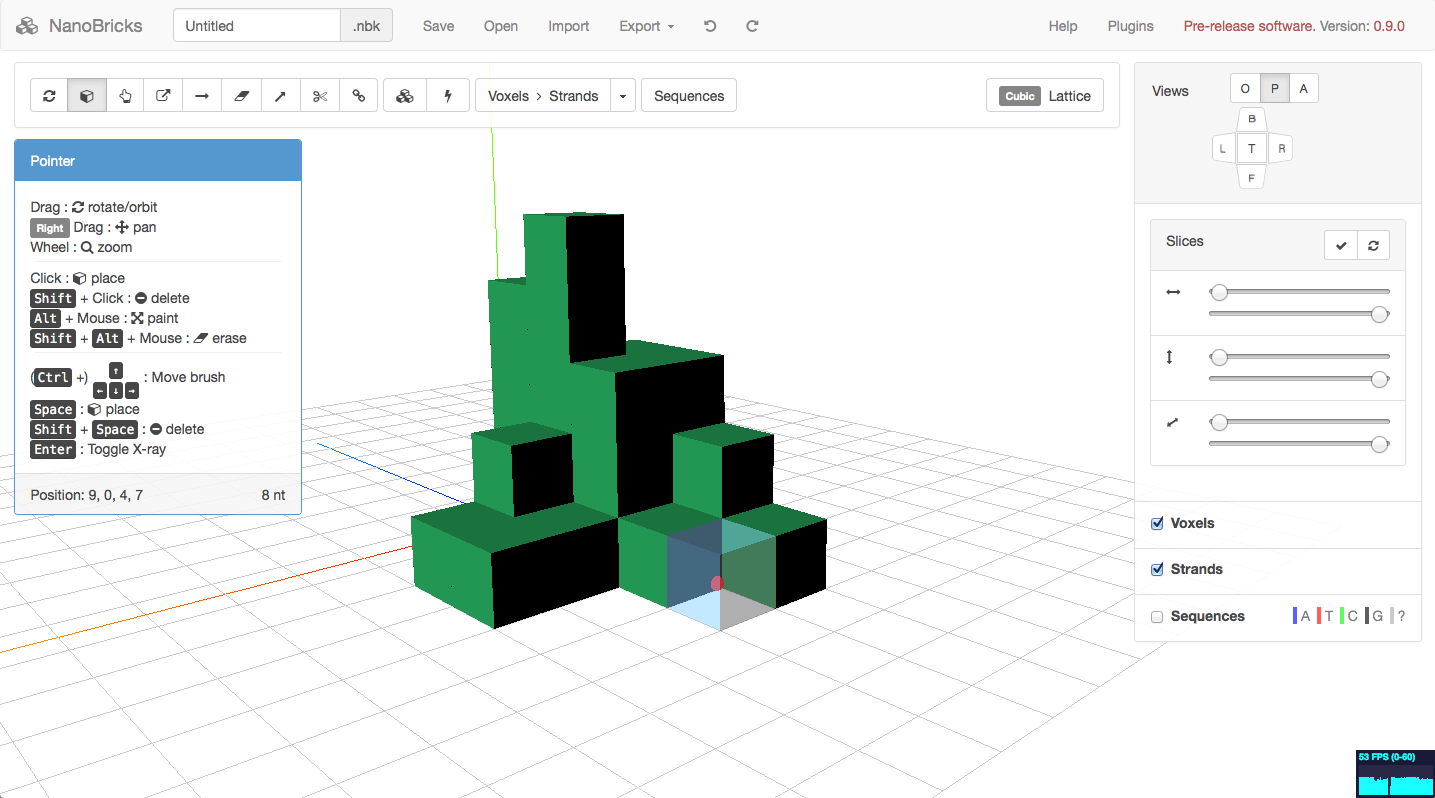
\includegraphics[width=\linewidth]{nanoBricks.png}
  \caption{Screenshot of NanoBricks, a voxel-based design tool for DNA Bricks by the Peng Yin Lab.}
  \label{fig:nanoBricks}
\end{figure}

\href{http://cadnano.org/}{CaDNAno} is a DNA origami design tool originally written by Douglas et al.\cite{Douglas2009}, and later adopted by Autodesk as a plugin for Maya.  It allows users to design 2D and 3D DNA origami structures based on one or several "scaffold" strands folded into a particular shape by many "staple" strands.  Structures are designed on a regular square or honeycomb lattice, though, single nucleotide insertions and deletions can be added to create programmable bending\cite{Dietz2009}\cite{Kim2012}.\\

\href{http://cando-dna-origami.org/}{Cando} is a DNA origami simulation package developed and maintained by Mark Bathe's group at MIT.  It models double stranded DNA as a homogeneous elastic rod with elastic constants and other physical parameters drawn from empirical measurements\cite{Peters2014}.  Crossovers between double stranded segments are modeled as elastic constraints on the rod elements.  Though these crossovers may deform double stranded segments out of a regular lattice configuration (which they are typically designed in) to form complex 3D geometries, simulated CanDo results show good agreement with experimental results\cite{Kim2012a}.  CanDo supports formats from CaDNAno and other DNA design environments.
\\

\href{http://yin.hms.harvard.edu/bricks/try/}{Nanobricks} is a voxel-based design tool for DNA Bricks.  Nanobricks allows a user to design nano-scale structures with voxels on a cubic lattice, and voxel-based designs are converted to sequences and exported as a text file.  Though Nanobricks offers less flexibility than caDNAno (eg it does not allow for out of lattice bending designs), it is significantly easier to design valid structures for a novice user.  Direct integration with CanDo is forthcoming.
\\

\subsection{Physics-Based Tools}

\begin{figure}
  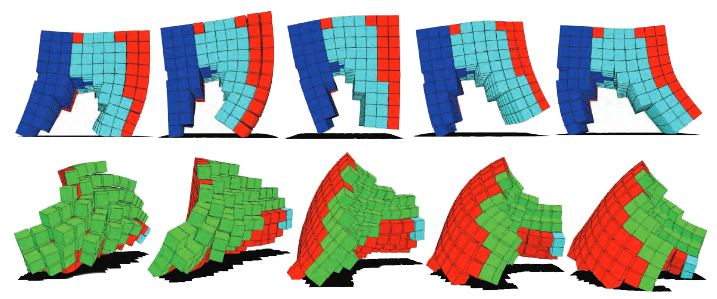
\includegraphics[width=\linewidth]{voxcadWalkers.png}
  \caption{Example gaits of two locomotion robots built from four material types in VoxCAD\cite{Cheney2013b}.  \textit{Image Credit: Cheney et al. 2013}}
  \label{fig:voxcadWalkers}
\end{figure}

\href{http://www.voxcad.com/}{Voxcad} is a physics-based design and dynamic simulation environment by Jonathan Hiller where a user designs virtual soft robots from four block types - two active and two passive\cite{Hiller2014a}.  Though the passive block types descended from a simulation of multimaterial 3D printed voxels, the active block types are not easily fabricated and actuated\cite{Hiller2012} and have not been rigorously evaluated.  Work into the optimization of theoretical locomotion systems in this virtual design space have been explored (Fig: \ref{fig:voxcadWalkers})\cite{Cheney2013b}\cite{Cheney2013}\cite{Cheney2015}.
\\

\begin{figure}
  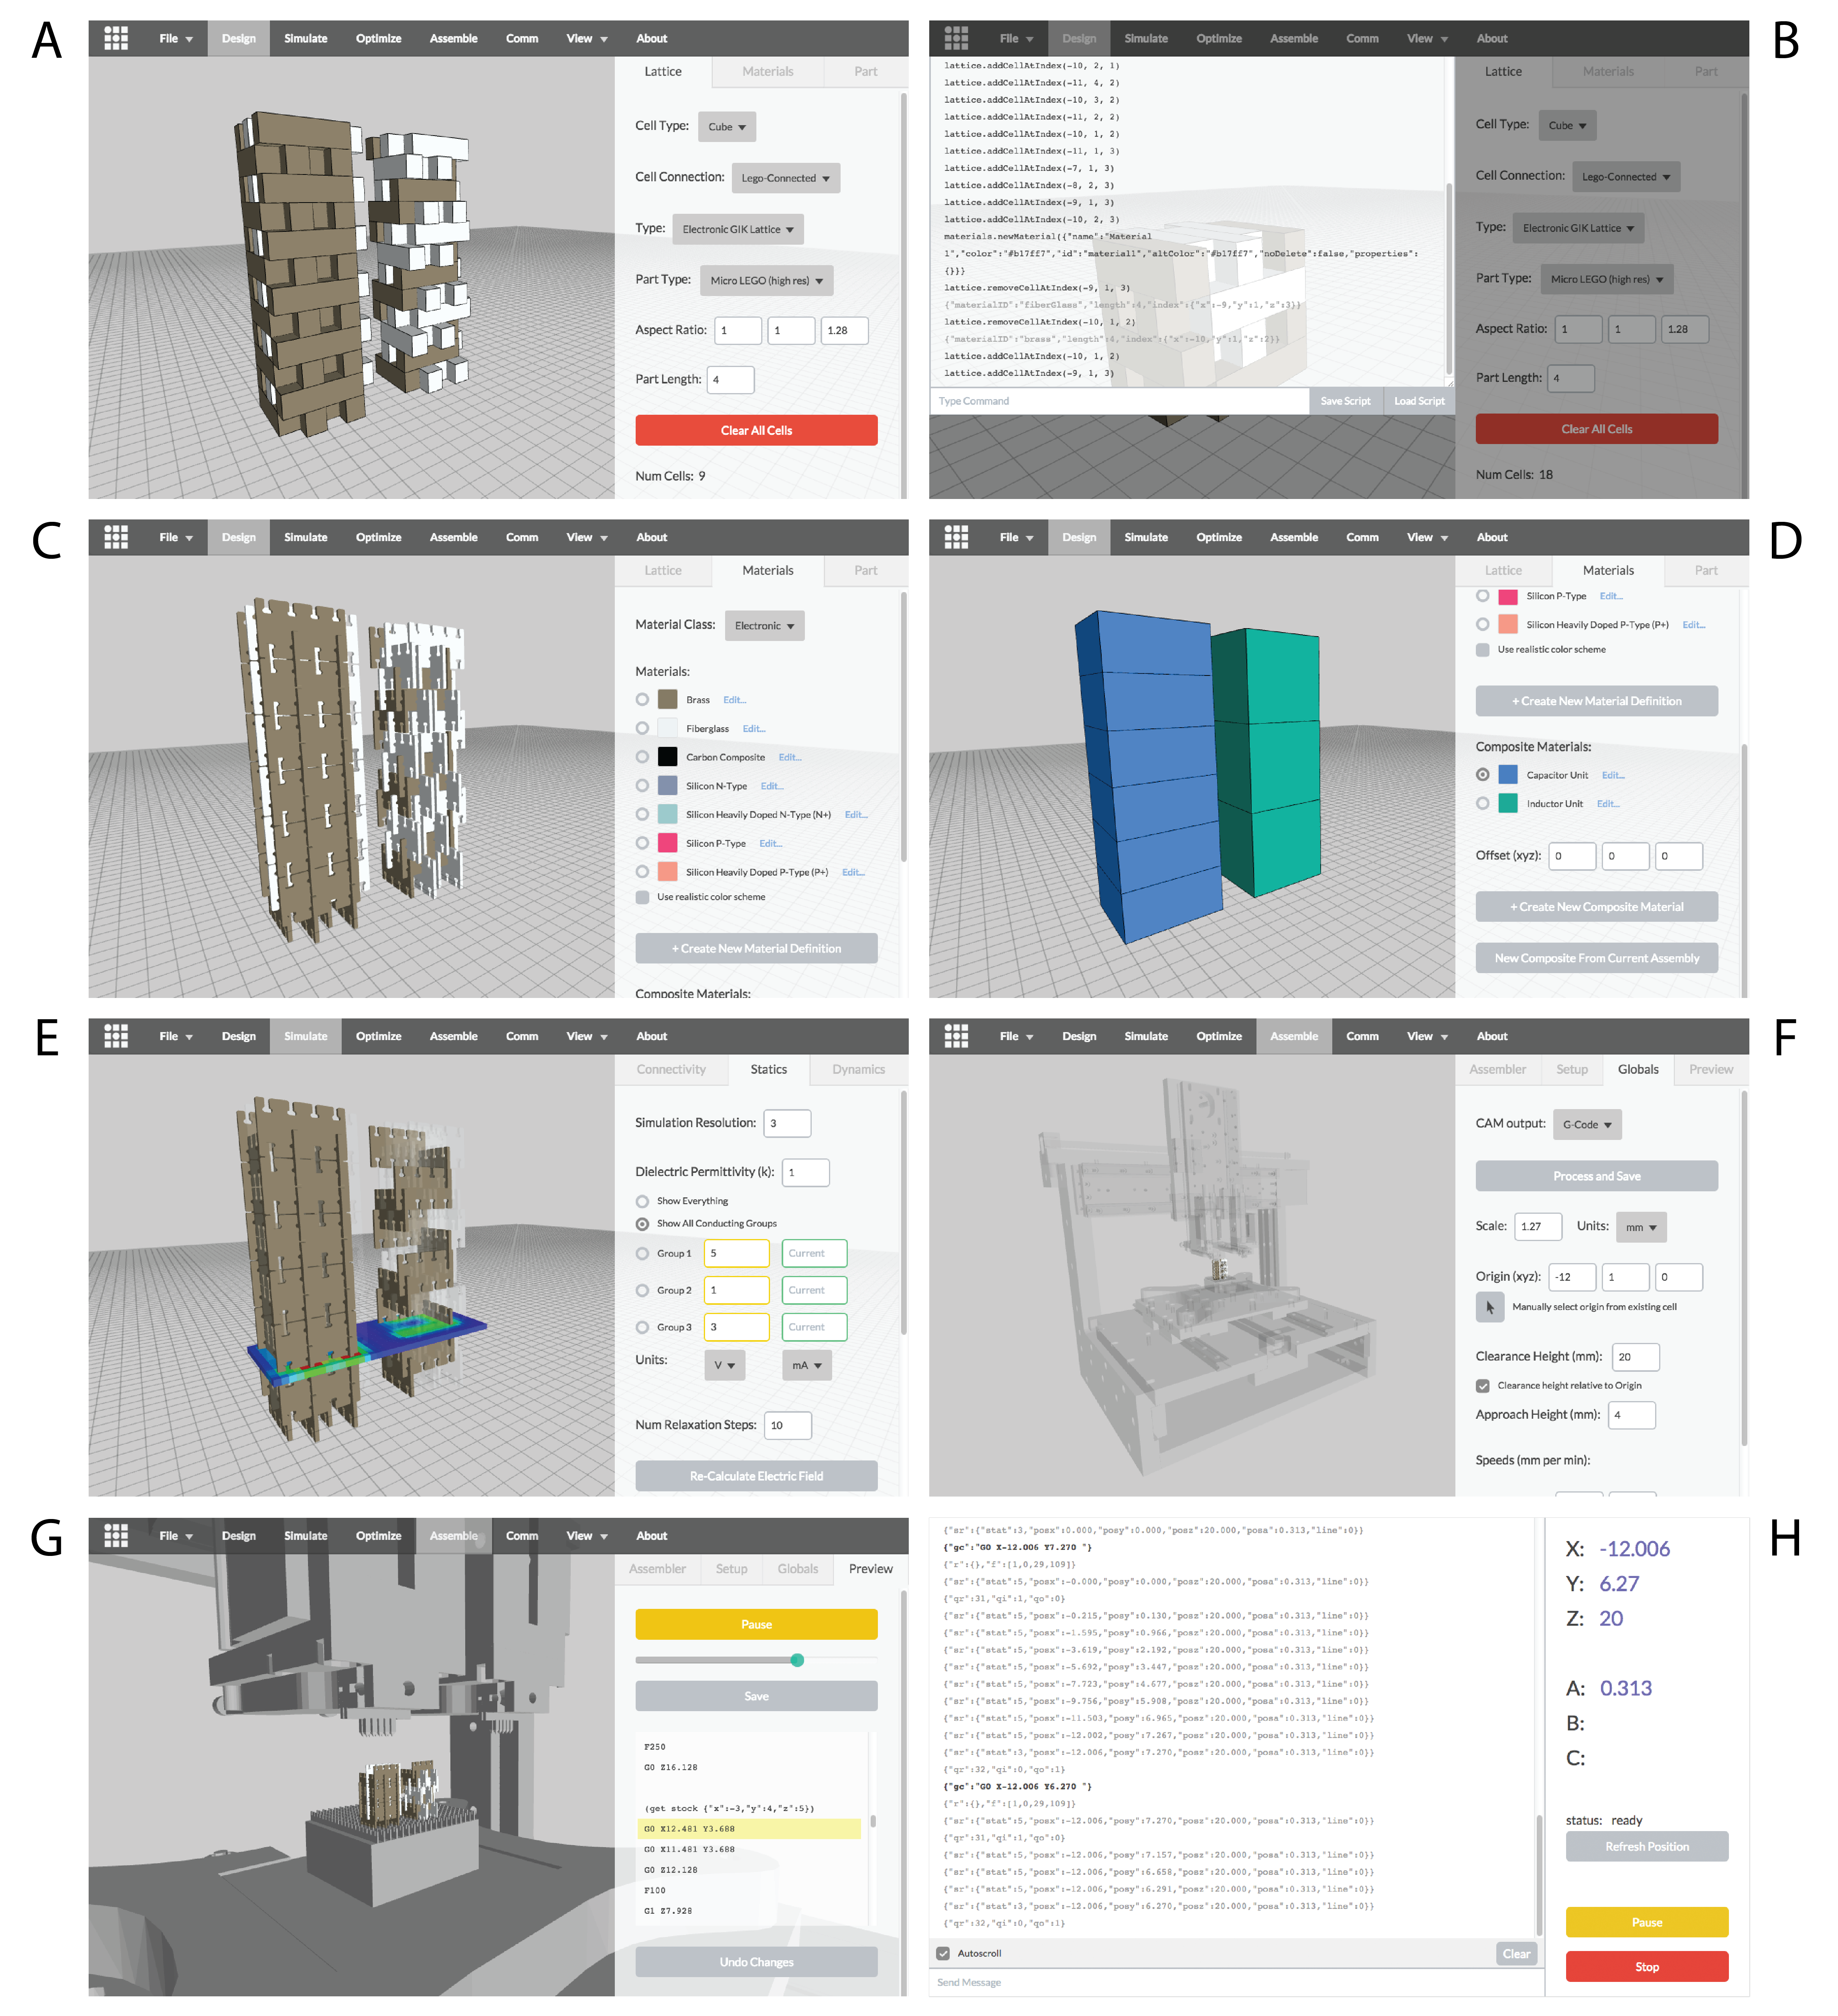
\includegraphics[width=\linewidth]{20151215DMDesignscreenshotsx8.png}
  \caption{Screenshots of my current work with DMDesign, a CAD/Simulation/CAM software package for Digital Materials. Structures are designed from multiple materials in a hierarchical \textbf{(D)}, 3D CAD interface or scripting API \textbf{(B)} that can toggle between a geometric and parts design representation \textbf{(A, C)}. Simulation of the potential field around conducting elements of an LC structure designed from conductive and insulating parts \textbf{(E)}. Path planning and visualization of the assembly process \textbf{(F, G)} and serial interface with machine \textbf{(H)}.}
  \label{fig: designAssemblyGUIWide}
\end{figure}
\href{http://dma.cba.mit.edu/dmdesign/}{DMDesign} is a CAD/CAM environment for digital materials I've been developing that supports the research efforts into part and assembler design at CBA (Fig \ref{fig: designAssemblyGUIWide}).  In DMDesign, users design structures in a virtual 3D environment from many material types, plan out the assembly of a design by a robotic assembler, and communicate in realtime with hardware to physically realize the design\cite{LangfordWillGhassaeiAmandaGershenfeld2016}.  By abstracting the geometry of the lattice from its decomposition into parts and implementing many lattice types in the CAD workflow, users can design structures ranging from nano to meter scale for a variety of application spaces.

}

\section{Self-Assembling Systems}

\subsection{Biological Systems}

\subsection{Modular Robotics}

\section{Micro Robotics}

%%% This is an example first chapter.  You should put chapter/appendix that you
%% write into a separate file, and add a line \include{yourfilename} to
%% main.tex, where `yourfilename.tex' is the name of the chapter/appendix file.
%% You can process specific files by typing their names in at the 
%% \files=
%% prompt when you run the file main.tex through LaTeX.

\singlespacing{


\chapter{Simulation Engine}

\section{Material Types}

We chose a relatively small basis set of material types which cover a range of desirable material properties for actuation and control.  The list of materials and a qualitative comparison of their properties is given in Table \ref{tab:materialTypes}.

\renewcommand{\arraystretch}{1.5}
%http://tex.stackexchange.com/questions/98388/how-to-make-table-with-rotated-table-headers-in-latex
\begin{table}[h] \label{tab:materialTypes}
    \centering
    \caption{Basis Set of Material Types.}
\begin{tabular}{ll | m{4cm} | *{7}{c} }
    \\
    \multicolumn{2}{c}{Function}  & \multicolumn{1}{c}{Example Materials}
        & \mcrot{1}{l}{60}{Cost} & \mcrot{1}{l}{60}{Strength} & \mcrot{1}{l}{60}{Stiffness} & \mcrot{1}{l}{60}{Fracture Resistance} & \mcrot{1}{l}{60}{Heat Resistance} & \mcrot{1}{l}{60}{Density} & \mcrot{1}{l}{60}{Magnetic Coercivity}\\
    \midrule \midrule

    \multirow{4}{*}{\rotatebox{90}{\textbf{\small{\hspace{17pt}Structural}}}}
    & Insulating & Plastics&
        x & x & x & xxx & x & xxx & -\\
    & Non-Insulating &   Metals  &
        xx & xxx & xxx & xx & xxx 
        & xx & -\\
    & Heat-Resistant&     Inconel, Alumina&
        xxxx &xx &xxxx &x &xxxx &xx & -\\
    \midrule
    \multirow{4}{*}{\rotatebox{90}{\textbf{\small{\hspace{18pt}Flexible}}}}
    & Insulating & Rubber
        & x & x & - & - & x 
        & - & x \\
    & Conductive & Metal wire   
        & x & x & - & - & x 
        & - & x\\
    & Hinge&    Metal flexure   
        & - & - & x & - & - 
        & - & -\\
        
      \midrule
     \multirow{4}{*}{\rotatebox{90}{\textbf{\small{\hspace{14pt}Conductive}}}}
    & General Purpose & Copper
        & x & x & - & - & x 
        & - & x\\
    & Lightweight &    Aluminum    
        & - & - & x & - & - 
        & - & -\\
    & Resistive&    Carbon-filled ceramic
        & - & - & x & - & - 
        & - & -\\
        
        
        \midrule
     \multirow{4}{*}{\rotatebox{90}{\textbf{\small{\hspace{16pt}Magnetic}}}}
    & Hard & NdFeB (neodymium)
        & x & x & - & - & x 
        & - & x\\
    & Soft &    AlNiCo   
        & - & - & x & - & - 
        & - & -\\
    & Ferromagnetic &    Iron     
        & - & - & x & - & - 
        & - & - \\
        
          \midrule
     \multirow{4}{*}{\rotatebox{90}{\textbf{\small{\hspace{50pt}Actuators}}}}
    & Piezoelectric & PZT (lead zirconate titanate)
        & x & x & - & - & x 
        & - & x\\
    & Heat Actuator &    Parrafin Wax
        & - & - & x & - & - 
        & - & -\\
        
         \midrule
     \multirow{4}{*}{\rotatebox{90}{\textbf{\small{Logic}}}}
    & NMOS & Silicon MOSFET
        & x & x & - & - & x 
        & - & x\\
    & PMOS &    Silicon MOSFET
        & - & - & x & - & - 
        & - & -\\
    & Diode &    Silicon     
        & - & - & x & - & - 
        & - & - \\
    & Zener Diode &    Silicon     
        & - & - & x & - & - 
        & - & - \\
        
        
        
    \bottomrule
\end{tabular}
\end{table}


\section{Hello World}

Before diving into more complex models, I wrote a "hello world" simulation engine to better understand how all the pieces of simulation (electronic, mechanical, and magnetic) would come together.

\subsection{Simple Mechanical Simulation}

I started with a simple dynamic mechanical model where the forces acting on each cell in the lattice are computed based on local interactions with its six neighbors and gravity.  In the model, virtual springs and dampers constrain translational and rotational motion of a cell relative to its neighbors (Fig \ref{fig: helloWorldLocalInteraction}).  At each time step all forces acting on each cell in the lattice are summed and the position, orientation, and translational and rotational velocities of the cell are solved by Euler integration.  All cells are updated synchronously, so the order of evaluation of the cells is not important.  All physical constants used in these calculations (mass of the cell, moment of inertia, spring stiffness, damping coefficient) are derived from the geometry and material properties of each cell.\\

In this scheme, the total force applied to the center of mass of a cell is given by:

\[ F_{total} =  \vec{f}_g+ \sum_{neighbors} \vec{f}_{neighbor}\]

With the total torque applied to the cell is given by the sum of the torques applied by its neighbors:

\[ T_{total} =  \sum_{neighbors} \tau_{neighbor} \]


\begin{figure}
  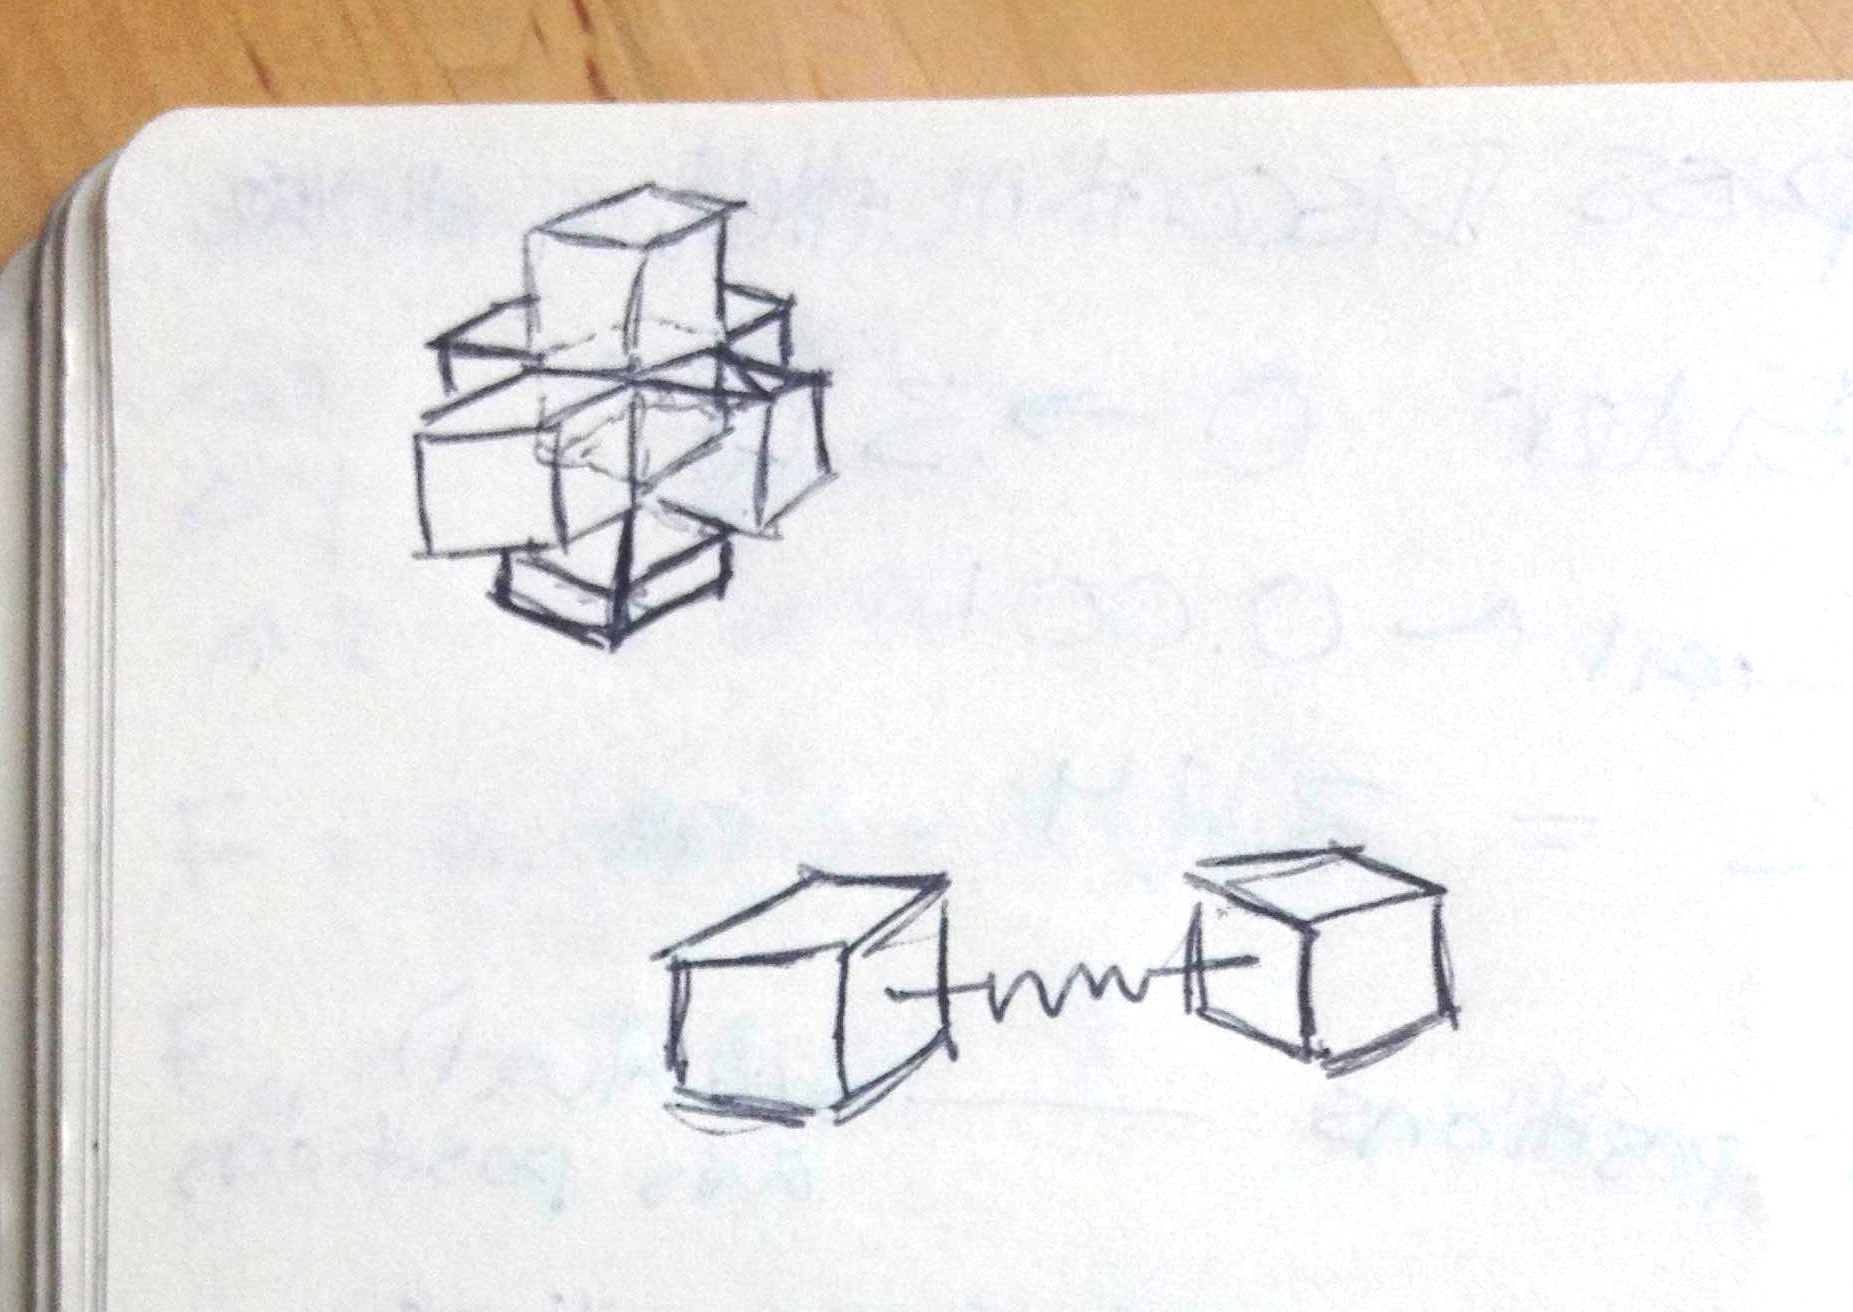
\includegraphics[width=\linewidth]{helloWorldLocalInteraction.png}
  \caption{REPLACE THIS Each cell is face-connected to its six local neighbors \textbf{(A)}.  Interaction between neighbors is modeled with springs and dampers constraining translational and rotational motion \textbf{(B)}.}
  \label{fig: helloWorldLocalInteraction}
\end{figure}

%To understand how the translational spring forces were calculated between two adjacent cells, consider the 2D case illustrated in Fig \ref{fig: helloWorldSpringSetup}.  The cells are attached by a spring with nominal length $\ell$.  Under displacement $\Delta x$ and $\Delta y$, the distance vector from cell A to cell B is given by $\vec{D}$.  Then $\Delta \ell$, the displacement of the spring from its nominal length, is given by:\\
%
%\[ \Delta \ell = \| D\| - \ell\]
%
%The force, $\vec{f}_{AB}$, exerted on cell A by a spring with stiffness $k$ is oriented in the same direction as $\vec{D}$:
%
%\[ \vec{f}_{AB} =  k (\hat{D} \Delta \ell) = k\hat{D} (\|D\| - \ell)\]
%
%An equal and opposite force, $\vec{f}_{BA}$, is applied to cell B by the spring:
%
%\[ \vec{f}_{BA} = -k\hat{D} (\|D\| - \ell)\]
%
%\begin{figure}
%  \includegraphics[width=\linewidth]{helloWorldSpringSetup.png}
%  \caption{REPLACE THIS Cubes A and B connected by spring with nominal length $\ell$ \textbf{(A)}.  The cells are displaced by $\Delta x$ and $\Delta y$ \textbf{(B)}. Spring displacement $\Delta \ell$ along $\vec{D}$ \textbf{( C )}.  $\vec{f}_{AB}$ and $\vec{f}_{BA}$ are the resulting translational spring forces applied to cells A and B, respectively \textbf{(D)}.  Larger translational displacements between neighboring cells increase the amplitude of spring forces \textbf{(E)}.}
%  \label{fig: helloWorldSpringSetup}
%\end{figure}

To understand how the translational forces were calculated between two adjacent cells, consider the 2D case illustrated in Fig \ref{fig: helloWorldSpringSetup}.  The cells are attached to each other with nominal displacement $\vec{\ell}$ from the center of cell A to the center of cell B.  If we model a two dimensional spring damper system connecting the cells, then the force applied to cell A by cell B under additional displacement $\Delta x$ and $\Delta y$ is given by:

\[ \vec{f}_{AB} =   k\left[ \begin{array}{ccc}
\Delta x \\
\Delta y \end{array} \right] - d 
\left[ \begin{array}{ccc}
v_x\\
v_y\end{array} \right] 
 \]

where k is a spring stiffness, d is a damping coefficient, and $v$ is the velocity of cell A relative to cell B.  This equation is trivially extended to the three dimensional case:\\

\[ \vec{f}_{AB} =   k\left[ \begin{array}{ccc}
\Delta x \\
\Delta y\\
\Delta z \end{array} \right] - d 
\left[ \begin{array}{ccc}
v_x\\
v_y\\
v_z\end{array} \right] 
 \]

\begin{figure}
  \includegraphics[width=\linewidth]{helloWorldSpringSetup.png}
  \caption{REPLACE THIS Adjacent cells A and B connected with nominal displacement $\vec{\ell}$ \textbf{(A)}.  The cells are additionally displaced by $\Delta x$ and $\Delta y$ \textbf{(B)}. $\vec{f}_{AB}$ and $\vec{f}_{BA}$ are the resulting translational spring-damper forces applied to cells A and B, respectively \textbf{( C )}.}
  \label{fig: helloWorldSpringSetup}
\end{figure}


The stiffness $k$ and damping coefficient $d$ of the springs and dampers are determined from the material properties of the two cells.  In the case that the two cells have different stiffnesses, a composite stiffness is calculated according to:

\[ k = \frac{2k_Ak_B}{k_A + k_B} \]

which is equivalent to two springs of half length in series.  Similarly, a composite damping coefficient is calculated by:\\

\[ d = \frac{2d_Ad_B}{d_A + d_B} \]

In addition to $\vec{f}_{AB}$, an equal and opposite force, $\vec{f}_{BA}$, is applied to cell B by the spring damper system (Fig \ref{fig: helloWorldSpringSetup} C):

\[ \vec{f}_{BA} =  -\vec{f}_{AB}\]

In addition to translational forces, neighboring cells apply torques to each other.  These torques result in rotational motion of a cell about its center of mass.  More on that soon.

%\begin{figure}
%  \includegraphics[width=\linewidth]{helloWorldSpringSetup.png}
%  \caption{REPLACE THIS Cubes A and B connected by spring with nominal displacement $\ell$ \textbf{(A)}.  The cells are further displaced by $\Delta x$ and $\Delta y$ \textbf{(B)}. Spring displacement $\Delta \ell$ along $\vec{D}$ \textbf{�}.  $\vec{f_{AB}}$ is the translational spring resulting force applied to cell A by the spring attached to cell B, force of gravity, $f_g$, also indicated \textbf{(D)}.}
%  \label{fig: helloWorldSpringRotSetup}
%\end{figure}









}

%%% This is an example first chapter.  You should put chapter/appendix that you
%% write into a separate file, and add a line \include{yourfilename} to
%% main.tex, where `yourfilename.tex' is the name of the chapter/appendix file.
%% You can process specific files by typing their names in at the 
%% \files=
%% prompt when you run the file main.tex through LaTeX.

\singlespacing{


\chapter{Micro Actuators}

\section{Overview}

 is given in Table \ref{tab:actuatorTypes}.

\renewcommand{\arraystretch}{1.5}
%http://tex.stackexchange.com/questions/98388/how-to-make-table-with-rotated-table-headers-in-latex
\begin{table}[h] \label{tab:actuatorTypes}
    \centering
    \caption{Micro-Actuation mechanisms comparison chart.}
\begin{tabular}{ll | *{7}{c} }
    \\
    \multicolumn{2}{c}{Name} 
        & \mcrot{1}{l}{60}{Cost} & \mcrot{1}{l}{60}{Density} & \mcrot{1}{l}{60}{Energy Density} & \mcrot{1}{l}{60}{Efficiency} & \mcrot{1}{l}{60}{Scaling} & \mcrot{1}{l}{60}{Strain} & \mcrot{1}{l}{60}{Etc}\\
    \midrule \midrule

    \multirow{4}{*}{\rotatebox{90}{\textbf{\small{\hspace{17pt}Electromagnetic}}}}
    & Solenoid&
        x & x & x & xxx & x & xxx & -\\
    & Voice-Coil  &
        xx & xxx & xxx & xx & xxx 
        & xx & -\\
    \midrule
    \multirow{4}{*}{\rotatebox{90}{\textbf{\small{\hspace{18pt}Electrostatic}}}}
    & Comb Drive
        & x & x & - & - & x 
        & - & x \\
        
      \midrule
     \multirow{4}{*}{\rotatebox{90}{\textbf{\small{\hspace{14pt}Piezo}}}}
    & PZT
        & x & x & - & - & x 
        & - & x\\
        
        \midrule
     \multirow{4}{*}{\rotatebox{90}{\textbf{\small{\hspace{16pt}Thermal}}}}
    & Paraffin Wax
        & x & x & - & - & x 
        & - & x\\
        
        
                \midrule
     \multirow{4}{*}{\rotatebox{90}{\textbf{\small{\hspace{16pt}Pnuematic}}}}
    & Air-Driven
        & x & x & - & - & x 
        & - & x\\
    & Fluid-Driven 
        & - & - & x & - & - 
        & - & -\\
        
        
    \bottomrule
\end{tabular}
\end{table}


\section{Electromagnetic}

\subsection{Solenoid}

\subsection{Voice Coil}

\section{Electrostatic}

\subsection{Electrostatic Comb Drive}

\section{Piezo}

\section{Thermal}

\subsection{Wax Actuator}

\section{Pneumatic}

\section{Ultrasonic}





}

%\appendix
%\chapter{Tables}

\begin{table}
\caption{Armadillos}
\label{arm:table}
\begin{center}
\begin{tabular}{||l|l||}\hline
Armadillos & are \\\hline
our	   & friends \\\hline
\end{tabular}
\end{center}
\end{table}

\clearpage
\newpage

%\chapter{Figures}

\vspace*{-3in}

\begin{figure}
\vspace{2.4in}
\caption{Armadillo slaying lawyer.}
\label{arm:fig1}
\end{figure}
\clearpage
\newpage

\begin{figure}
\vspace{2.4in}
\caption{Armadillo eradicating national debt.}
\label{arm:fig2}
\end{figure}
\clearpage
\newpage

%% This defines the bibliography file (main.bib) and the bibliography style.
%% If you want to create a bibliography file by hand, change the contents of
%% this file to a `thebibliography' environment.  For more information 
%% see section 4.3 of the LaTeX manual.
\begin{singlespace}
\renewcommand{\bibname}{References}
\bibliography{mendeley/ThesisWURL}
\bibliographystyle{customBibStyle}
\end{singlespace}

%%% This defines the bibliography file (main.bib) and the bibliography style.
%% If you want to create a bibliography file by hand, change the contents of
%% this file to a `thebibliography' environment.  For more information 
%% see section 4.3 of the LaTeX manual.
\begin{singlespace}
\renewcommand{\bibname}{External Media}
\begin{thebibliography}{1}

\bibitem{jifei}
\href{http://ou-jifei.com/}{Jifei Ou personal website}.  Images of multimaterial Objet print taken from \href{https://vimeo.com/127666944#t=89s}{Autodesk Pier 9 video}.

\bibitem{objet}
\href{http://www.stratasys.com/3d-printers/production-series/connex3-systems}{Objet Connex Multimaterial 3D Printer website}

\bibitem{minecraft}
\href{https://minecraft.net/}{Official Minecraft website}

\bibitem{redstoneCircuit}
\href{http://minecraft.gamepedia.com/Redstone_circuit}{Redstone Circuit - Minecraft Wiki}

\end{thebibliography}
\end{singlespace}

\end{document}

